% ============================================================
%  TESIS  -  Documento maestro (estructura modular)
%
%  Escuela Profesional de Ingenieria Informatica y de Sistemas - UNSAAC
%  Titulo: Desarrollo de un sistema bidireccional de traduccion de voz
%          Quechua-Espanol mediante arquitecturas de transformadores
%          multimodales para consultas medicas en Cusco.
%
%  Estructura por capitulos (plantilla UNSAAC):
%    I.   Introduccion (sistema de 6 bloques)   -> 04AspectosGenerales
%    II.  Marco teorico y estado del arte        -> 05MarcoTeorico
%    III. Metodologia de la investigacion        -> 06Metodologia
%    IV.  Experimentacion y Resultados (EDA)      -> 06bExperimentacion
%    V.   Estudio de factibilidad                -> 07Factibilidad
%    VI.  Aspectos administrativos               -> 08Administrativos
%    + Bibliografia y Anexos                      -> 09, 10
%
%  Compilar:  pdflatex main -> biber main -> pdflatex main -> pdflatex main
% ============================================================
\documentclass[12pt,a4paper]{article}
% ============================================================
%  00preambulo.tex  -  Preambulo consolidado de la Tesis
%  (APA7 + espanol + graficos + matematica + matriz apaisada)
%  Compilar desde main.tex:  pdflatex -> biber -> pdflatex -> pdflatex
% ============================================================

% ---- Codificacion e idioma ----
\usepackage[utf8]{inputenc}
\usepackage[T1]{fontenc}
\usepackage{lmodern}
\usepackage[spanish,es-tabla]{babel}
\usepackage{csquotes}

% ---- Geometria (margenes tipo tesis) ----
\usepackage[a4paper,left=3cm,right=2.5cm,top=2.5cm,bottom=2.5cm]{geometry}

% ---- Interlineado 1.5 ----
\usepackage{setspace}
\onehalfspacing

% ---- Tipografia de titulos (se re-define mas abajo para APA7) ----
\usepackage{titlesec}

% ---- Tablas y figuras ----
\usepackage{graphicx}
\usepackage{booktabs}
\usepackage{array}
\usepackage{multirow}
\usepackage{tabularx}
\usepackage{float}
\usepackage[font=small,labelfont=bf]{caption}

% ---- Matematica (atencion, perdida, flujo de datos de la cascada) ----
\usepackage{amsmath}

% ---- Pagina apaisada para la matriz de consistencia ----
\usepackage{pdflscape}

% ---- Color de celdas / rampas ----
\usepackage{colortbl}

% ---- Graficos vectoriales (pgfplots / tikz) ----
\usepackage{pgfplots}
\pgfplotsset{compat=1.18}
\usepackage{tikz}
\usetikzlibrary{shapes.geometric,arrows.meta,positioning,calc}

% ---- Colores base ----
\usepackage{xcolor}
\definecolor{azulUNSAAC}{RGB}{0,71,133}
\definecolor{grisSuave}{RGB}{240,240,240}

% ---- Rutas de imagenes (logo, figuras) ----
\graphicspath{{imagenes/}{./}{../}}

% ---- Bibliografia APA7 (biblatex + biber) ----
\usepackage[
  backend=biber,
  style=apa,
  sortcites=true,
  sorting=nyt,
  language=spanish
]{biblatex}
\DeclareLanguageMapping{spanish}{spanish-apa}
% Fuentes: referencias generales (raiz del repo) y antecedentes de la revision.
\addbibresource{../referencias.bib}
\addbibresource{antecedentes.bib}

% ---- Listas e indices (tocloft ANTES de hyperref) ----
\usepackage{longtable}
\usepackage{algorithm}
\usepackage{algpseudocode}
\usepackage{tocloft}

% ---- Hipervinculos ----
\usepackage[hidelinks]{hyperref}
\hypersetup{
  colorlinks=true,
  linkcolor=black,
  citecolor=azulUNSAAC,
  urlcolor=azulUNSAAC
}

% ---- Icono ORCID ----
\usepackage{orcidlink}

% ---- Sangria de primer parrafo ----
\usepackage{indentfirst}

% ============================================================
%  Colores de la "ecuacion universal" del titulo (cafe/rojo/verde)
%  Esquema estandarizado (marco del docente): el titulo se descompone en tres
%  componentes, cada uno con un color fijo reutilizable en todo el proyecto.
% ============================================================
\definecolor{colProceso}{RGB}{122,66,20}   % cafe  -> Proceso / Accion
\definecolor{colMetodo}{RGB}{176,42,42}     % rojo  -> Tecnologia / Metodo
\definecolor{colContexto}{RGB}{31,110,54}   % verde -> Contexto / Aplicacion

% ============================================================
%  CORRECCIONES A OBSERVACIONES (revision del asesor)
% ============================================================
\definecolor{verdeOK}{RGB}{13,124,51}
% ---- Interruptor de versi{\'o}n ----
%  \docentetrue  = versi{\'o}n DOCENTE: nota inicial + cambios de la observaci{\'o}n 3
%                  (precisi{\'o}n del m{\'e}todo en el t{\'i}tulo) resaltados en VERDE.
%  \docentefalse = versi{\'o}n JURADO: todo en negro, sin nota ni resaltados.
\newif\ifdocente
\docentetrue
\ifdocente
  \newcommand{\obstitulo}[1]{\textcolor{verdeOK}{#1}}% observaci{\'o}n 3: t{\'i}tulo/m{\'e}todo
\else
  \newcommand{\obstitulo}[1]{#1}
\fi
% R1 consolidado: correcciones de la 1a ronda en NEGRO (texto normal).
\newcommand{\nuevo}[1]{#1}
\newenvironment{bloqueNuevo}{\par}{\par}
% R2 (2a ronda): aceptada; en NEGRO (texto normal).
\newcommand{\obsdos}[1]{#1}
\newenvironment{bloqueObsDos}{\par}{\par}
% R3: integrada al texto en NEGRO (versi{\'o}n para el jurado, sin resaltar correcciones).
\newcommand{\obstres}[1]{#1}
\newenvironment{bloqueObsTres}{\par}{\par}
% Mejoras propias de rigor (NO son una ronda del asesor): quedan en NEGRO (texto normal),
% integradas al documento como el resto. El macro se conserva por si luego se desea resaltar.
\newcommand{\obscuatro}[1]{#1}
\newenvironment{bloqueObsCuatro}{\par}{\par}

% ---- APA 7: numero y titulo ENCIMA de tablas y figuras; Nota al pie ----
\captionsetup{labelsep=newline,labelfont=bf,textfont=it,
              justification=raggedright,singlelinecheck=false}
\captionsetup[table]{position=above,skip=4pt}
\captionsetup[figure]{position=above,skip=6pt}
\newcommand{\notaAPA}[1]{\par\vspace{2pt}%
  \begin{minipage}{\linewidth}\footnotesize\textit{Nota.} #1\end{minipage}\par}

% ---- Estilo de tabla del proyecto (APA: cabecera negra sin relleno) ----
\newcommand{\hdr}[1]{\textbf{#1}}
\newcommand{\celnivel}[1]{\textbf{#1}}

% ---- Enlaces internos: siglas (quz/quy) y terminos del glosario ----
\DeclareRobustCommand{\sig}[1]{\hyperlink{sig:#1}{\texttt{#1}}}
\DeclareRobustCommand{\glo}[2]{\hyperlink{glo:#1}{#2}}
\newcommand{\destino}[1]{\hypertarget{#1}{}}

% ---- APA 7: encabezados ----
\titleformat{\section}[display]{\normalfont\Large\bfseries\filcenter}{Cap{\'i}tulo~\thesection}{0.3em}{}
\titleformat{name=\section,numberless}{\normalfont\Large\bfseries\filcenter}{}{0pt}{}
\titleformat{\subsection}{\normalfont\large\bfseries}{\thesubsection}{1em}{}
\titleformat{\subsubsection}{\normalfont\normalsize\bfseries\itshape}{\thesubsubsection}{1em}{}

% ---- Rampa estandar de los graficos: azul claro -> navy -> turquesa -> verde ----
\definecolor{g1}{HTML}{8AC4E6}
\definecolor{g2}{HTML}{66AEDA}
\definecolor{g3}{HTML}{4294CC}
\definecolor{g4}{HTML}{2E6DA0}
\definecolor{g5}{HTML}{1E4870}
\definecolor{g6}{HTML}{1F6476}
\definecolor{g7}{HTML}{229184}
\definecolor{g8}{HTML}{27A597}
\definecolor{g9}{HTML}{40B183}
\definecolor{g10}{HTML}{59BD6F}
\definecolor{g11}{HTML}{6AC362}
\definecolor{g12}{HTML}{7BC95A}

% ---- Numeracion por capitulos (I, II, ...) y subsecciones (2.1, 2.1.1) ----
\renewcommand{\thesection}{\Roman{section}}
\renewcommand{\thesubsection}{\arabic{section}.\arabic{subsection}}
\renewcommand{\thesubsubsection}{\arabic{section}.\arabic{subsection}.\arabic{subsubsection}}
\setcounter{secnumdepth}{3}
\setcounter{tocdepth}{3}

% ---- Nombres en espanol de los indices ----
\addto\captionsspanish{\renewcommand{\contentsname}{\'Indice general}}
\floatname{algorithm}{Algoritmo}
\renewcommand{\listalgorithmname}{\'Indice de algoritmos}

% ---- Indice de ecuaciones (lista propia via tocloft) ----
\newlistof{ecuaciones}{loe}{\'Indice de ecuaciones}
\newcommand{\regecuacion}[1]{%
  \addcontentsline{loe}{ecuaciones}{\protect\numberline{\theequation}#1}}
\let\cftecuacionesfont\cfttabfont
\let\cftecuacionespagefont\cfttabpagefont
\setlength{\cftecuacionesindent}{\cfttabindent}
\setlength{\cftecuacionesnumwidth}{\cfttabnumwidth}

% ---- Paginacion APA 7: numero en la esquina SUPERIOR DERECHA ----
\usepackage{fancyhdr}
\pagestyle{fancy}
\setlength{\headheight}{14.5pt}
\fancyhf{}
\fancyhead[R]{\thepage}
\renewcommand{\headrulewidth}{0pt}
\fancypagestyle{plain}{%
  \fancyhf{}%
  \fancyhead[R]{\thepage}%
  \renewcommand{\headrulewidth}{0pt}%
}


% ============================================================
%  COMPILACION POR CAPITULOS (ver instrucciones mas abajo)
%  Descomenta \includeonly y deja SOLO el/los capitulo(s) que
%  quieras compilar. Comentalo del todo para compilar la tesis
%  completa. La numeracion y las referencias se mantienen
%  gracias a los .aux de cada capitulo.
%
%    \includeonly{partes/04AspectosGenerales}   % solo Cap. I
%    \includeonly{partes/05MarcoTeorico}        % solo Cap. II
% ============================================================
%\includeonly{partes/04AspectosGenerales}

\begin{document}

% ---- Preliminares (siempre \input: no son capitulos) ----
% ================= CARÁTULA (plantilla UNSAAC) =================
% Sin ancla de p{\'a}gina en la car{\'a}tula para evitar el choque de destino
% "page.1" con la primera p{\'a}gina ar{\'a}biga del cuerpo.
\hypersetup{pageanchor=false}
\newlength{\tesisx}
\begin{titlepage}
\centering
\singlespacing

% ---- Encabezado institucional (negro, negrita) ----
{\normalsize\bfseries UNIVERSIDAD NACIONAL DE SAN ANTONIO ABAD DEL CUSCO\par}
\vspace{0.35cm}
{\normalsize\bfseries FACULTAD DE INGENIER{\'I}A EL{\'E}CTRICA, ELECTR{\'O}NICA,\\ INFORM{\'A}TICA Y MEC{\'A}NICA\par}
\vspace{0.35cm}
{\normalsize\bfseries ESCUELA PROFESIONAL DE INGENIER{\'I}A INFORM{\'A}TICA Y DE SISTEMAS\par}
\vspace{0.7cm}

% ---- Escudo ----
\IfFileExists{imagenes/logo_unsaac.png}{
\includegraphics[width=3.6cm]{imagenes/logo_unsaac.png}}{%
  \IfFileExists{../logo_unsaac.png}{
\includegraphics[width=3.6cm]{../logo_unsaac.png}}{}}
\vspace{0.8cm}

% ---- Tipo de documento ----
{\bfseries TESIS\par}
\vspace{0.5cm}

% ---- T{\'i}tulo dentro de un recuadro de esquinas redondeadas ----
\begin{tikzpicture}
  \node[draw=black, line width=0.6pt, rounded corners=12pt, inner sep=12pt,
        text width=0.82\linewidth, align=center, font=\bfseries\small]{%
    \textcolor{colProceso}{DESARROLLO DE UN SISTEMA BIDIRECCIONAL DE TRADUCCI{\'O}N DE VOZ
    QUECHUA--ESPA{\~N}OL} \textcolor{colMetodo}{MEDIANTE ARQUITECTURAS DE
    TRANSFORMADORES MULTIMODALES} \textcolor{colContexto}{PARA CONSULTAS
    M{\'E}DICAS EN CUSCO}};
\end{tikzpicture}\par

\vspace{0.5cm}

% ---- Datos: en negro, el bloque empieza donde empieza la palabra TESIS ----
%  (TESIS esta centrada: su borde izquierdo = (textwidth - ancho de "TESIS")/2)
\settowidth{\tesisx}{\normalsize\bfseries TESIS}%
\begin{flushleft}
\hspace*{\dimexpr0.5\textwidth-0.5\tesisx\relax}%
\begin{minipage}{\dimexpr0.5\textwidth+0.5\tesisx\relax}
\raggedright\fontsize{9}{11}\selectfont
{\bfseries PRESENTADO POR:}\\[4pt]
Br. ALAIN ARMANDO CONDORI CONTRERAS\\[4pt]
C{\'O}DIGO: 021501\\[16pt]
{\bfseries PARA OPTAR AL T{\'I}TULO PROFESIONAL DE}\\
{\bfseries INGENIERO INFORM{\'A}TICO Y DE SISTEMAS}\\[16pt]
{\bfseries ASESOR:}\\[4pt]
Mtro. Ing. RA{\'U}L HUILLCA HUALLPARIMACHI
\end{minipage}%
\end{flushleft}

\vspace{1.6cm}
{\bfseries CUSCO - PER{\'U}\par}
\vspace{0.2cm}
{\bfseries 2026\par}
\end{titlepage}
        % Caratula
% ================= DEDICATORIA =================
% Mismo formato que el PDF de referencia (253T20260080_TC.pdf, pag. 5):
% titulo a la derecha en negrita grande, texto en cursiva con interlineado
% amplio en un bloque desplazado a la derecha y el nombre del autor al final.
\clearpage
\thispagestyle{empty}

\vspace*{0.30\textheight}

{\hfill\Large\bfseries Dedicatoria\par}

\vspace{1.4cm}

\hfill
\begin{minipage}{0.68\textwidth}
  \itshape\setstretch{1.7}
  A Dios, por guiarme y darme la fortaleza necesaria en cada paso de este
  camino.

  A mis padres, por ser mi mayor inspiraci{\'o}n; su esfuerzo, su amor y sus
  ense{\~n}anzas hacen posible este logro y siguen siendo mi gu{\'i}a.

  A mis hermanos, por su compa{\~n}{\'i}a constante y su aliento en todo
  momento.\par

  \vspace{1.1cm}
  \normalfont\hfill Alain\par
\end{minipage}
\clearpage
    % Dedicatoria

% Preliminares en n{\'u}meros romanos (Resumen = p{\'a}gina I); la car{\'a}tula no se numera.
\pagenumbering{Roman}
\hypersetup{pageanchor=true}

% ================= RESUMEN =================
\section*{Resumen}
\addcontentsline{toc}{section}{Resumen}
\singlespacing\noindent
En la regi{\'o}n Cusco, m{\'a}s del 55\,\% de la poblaci{\'o}n tiene el quechua como lengua
materna y cerca de 70\,000 asegurados de EsSalud son quechuahablantes \parencite{essalud2023};
esta barrera idiom{\'a}tica afecta la calidad de la atenci{\'o}n en salud \parencite{begazo2026}.

El presente trabajo propone desarrollar y evaluar un sistema bidireccional de traducci{\'o}n de
voz Quechua--Espa{\~n}ol para consultas m{\'e}dicas, que encadena reconocimiento de voz (MMS),
traducci{\'o}n autom{\'a}tica (NLLB adaptado al quechua de Cusco, \sig{quz}) y s{\'i}ntesis de
voz (MMS-TTS) mediante el ajuste (\emph{fine-tuning}) de modelos preentrenados de c{\'o}digo
abierto \obstitulo{basados en arquitecturas de transformadores multimodales ---el est{\'a}ndar
actual para procesar voz y texto---}.

La salida por voz en ambos sentidos busca incluir a la poblaci{\'o}n quechuahablante con
baja o nula alfabetizaci{\'o}n. La validaci{\'o}n se realizar{\'a} con consultas simuladas, sin datos
reales de pacientes, midiendo precisi{\'o}n (WER, BLEU, chrF), calidad de voz (MOS) y percepci{\'o}n
de utilidad. Se espera aportar el primer corpus cl{\'i}nico Quechua--Espa{\~n}ol y evidencia
emp{\'i}rica sobre la viabilidad de estas tecnolog{\'i}as en el dominio sanitario andino.

\vspace{0.3cm}
\textit{Palabras clave:} \nuevo{Traducci{\'o}n autom{\'a}tica, Quechua, Procesamiento del
lenguaje natural, Comunicaci{\'o}n m{\'e}dico-paciente, Inclusi{\'o}n digital.}
\onehalfspacing

\ifdocente
\vspace{0.4cm}
\noindent\fcolorbox{verdeOK}{white}{\begin{minipage}{0.98\linewidth}\footnotesize
\textcolor{verdeOK}{\textbf{Nota de revisi{\'o}n.}} El texto en
\textcolor{verdeOK}{\textbf{verde}} corresponde a las \textbf{correcciones realizadas en respuesta a
la tercera observaci{\'o}n} del asesor: la precisi{\'o}n del m{\'e}todo en el t{\'i}tulo y en el
documento ---de \emph{aprendizaje profundo} a \textbf{arquitecturas de transformadores
multimodales}---, con su fundamentaci{\'o}n en el marco te{\'o}rico. Las observaciones previas ya
fueron integradas al texto.
\end{minipage}}
\fi

\newpage
\section*{Abstract}
\addcontentsline{toc}{section}{Abstract}
\singlespacing\noindent
In the Cusco region, more than 55\% of the population has Quechua as their mother tongue and
nearly 70{,}000 EsSalud insured members are Quechua speakers \parencite{essalud2023}; this language
barrier affects the quality of health care \parencite{begazo2026}.

This work proposes to develop and
evaluate a bidirectional Quechua--Spanish speech translation \emph{system} for medical consultations,
chaining speech recognition (MMS), machine translation (NLLB adapted to Cusco Quechua, \sig{quz}) and
speech synthesis (MMS-TTS) through the \emph{fine-tuning} of open-source pretrained models.

The
two-way voice output aims to include Quechua-speaking people with low or no literacy. Validation will
be carried out with simulated consultations, without real patient data, measuring accuracy (WER,
BLEU, chrF), voice quality (MOS) and perceived usefulness. The study is expected to contribute the
first clinical Quechua--Spanish corpus and empirical evidence on the feasibility of these
technologies in the Andean health domain.

\vspace{0.3cm}
\noindent\obsdos{\textit{Keywords:} Machine translation, Quechua, Natural language processing,
Doctor--patient communication, Digital inclusion.}
\onehalfspacing
         % Resumen y Abstract
\newpage
\tableofcontents                                   % Índice general

\clearpage
\addcontentsline{toc}{section}{\'Indice de figuras}
\listoffigures                                     % Índice de figuras

\clearpage
\addcontentsline{toc}{section}{\'Indice de tablas}
\listoftables                                      % Índice de tablas

\clearpage
\addcontentsline{toc}{section}{\'Indice de algoritmos}
\listofalgorithms                                  % Índice de algoritmos

\clearpage                                          % Índice de símbolos
\section*{\'Indice de s{\'i}mbolos}
\addcontentsline{toc}{section}{\'Indice de s{\'i}mbolos}
\begin{longtable}{@{}p{2.6cm} p{9cm} p{2.4cm}@{}}
\toprule\hdr{S{\'i}mbolo} & \hdr{Descripci{\'o}n} & \hdr{\obstres{P{\'a}gina}} \\
\midrule \endhead
$\alpha$ & Nivel de significancia estad{\'i}stica & \obstres{\pageref{sym:alpha}} \\
$N$      & Tama{\~n}o de muestra / n.\ de palabras de referencia & \obstres{\pageref{eq:wer}} \\
$\beta$  & Factor de ponderaci{\'o}n recall/precisi{\'o}n en chrF & \obstres{\pageref{eq:chrf}} \\
$S,D,I$  & Sustituciones, eliminaciones e inserciones (c{\'a}lculo del WER) & \obstres{\pageref{eq:wer}} \\
$\theta$ & Par{\'a}metros (pesos) del modelo ajustado por \emph{fine-tuning} & \obstres{\pageref{eq:perdida}} \\
$\mathcal{L}$ & Funci{\'o}n de p{\'e}rdida (entrop{\'i}a cruzada) del entrenamiento & \obstres{\pageref{eq:perdida}} \\
\bottomrule
\end{longtable}

\clearpage                                          % Índice de abreviaturas
\section*{\'Indice de abreviaturas}
\addcontentsline{toc}{section}{\'Indice de abreviaturas}
\begin{longtable}{@{}p{3cm} p{12cm}@{}}
\toprule\hdr{Sigla} & \hdr{Significado} \\
\midrule \endhead
IA      & Inteligencia artificial \\
PLN     & Procesamiento del lenguaje natural \\
ASR     & Reconocimiento autom{\'a}tico del habla (\emph{Automatic Speech Recognition}) \\
STT     & Voz a texto (\emph{Speech-to-Text}) \\
TTS     & S{\'i}ntesis de voz (\emph{Text-to-Speech}) \\
MT      & Traducci{\'o}n autom{\'a}tica (\emph{Machine Translation}) \\
MMS     & \emph{Massively Multilingual Speech} (Meta) \\
NLLB    & \emph{No Language Left Behind} (Meta) \\
WER     & Tasa de error de palabra (\emph{Word Error Rate}) \\
BLEU    & \emph{Bilingual Evaluation Understudy} \\
chrF    & \emph{Character n-gram F-score} \\
MOS     & \emph{Mean Opinion Score} \\
quz     & Quechua Collao / Cusco (c{\'o}digo ISO 639-3)\destino{sig:quz} \\
quy     & Quechua Ayacucho (c{\'o}digo ISO 639-3)\destino{sig:quy} \\
Transformer & \nuevo{Arquitectura de red neuronal basada en autoatenci{\'o}n (base de MMS/NLLB)} \\
INEI    & Instituto Nacional de Estad{\'i}stica e Inform{\'a}tica \\
EsSalud & Seguro Social de Salud del Per{\'u} \\
UNSAAC  & Universidad Nacional de San Antonio Abad del Cusco \\
\bottomrule
\end{longtable}

\clearpage                                          % Índice de ecuaciones
\section*{\'Indice de ecuaciones}
\addcontentsline{toc}{section}{\'Indice de ecuaciones}
\makeatletter\@starttoc{loe}\makeatother

\clearpage                                          % Glosario de términos
\section*{Glosario de t{\'e}rminos}
\addcontentsline{toc}{section}{Glosario de t{\'e}rminos}
\begin{longtable}{@{}p{3.6cm} p{11.4cm}@{}}
\toprule\hdr{T{\'e}rmino} & \hdr{Definici{\'o}n} \\
\midrule \endhead
Corpus                  & Conjunto estructurado de textos o grabaciones usado para entrenar o evaluar modelos.\destino{glo:corpus} \\
Fine-tuning             & Ajuste de un modelo preentrenado con datos de un dominio espec{\'i}fico.\destino{glo:finetuning} \\
Lengua de bajo recurso  & Idioma con escasez de datos digitales para entrenar modelos de PLN.\destino{glo:bajorecurso} \\
Modelo preentrenado     & Modelo entrenado sobre grandes vol{\'u}menes de datos, reutilizable mediante ajuste.\destino{glo:preentrenado} \\
Lengua polisint{\'e}tica & Lengua que concentra mucha informaci{\'o}n gramatical en una sola palabra, como el quechua.\destino{glo:polisintetica} \\
Pipeline                & Secuencia encadenada de etapas (voz $\to$ texto $\to$ traducci{\'o}n $\to$ voz).\destino{glo:pipeline} \\
\bottomrule
\end{longtable}

\clearpage
\setcounter{table}{0}\setcounter{figure}{0}
% Inicio del cuerpo: paginaci{\'o}n normal en ar{\'a}bigos desde 1 (APA).
\pagenumbering{arabic}
         % Indices, glosario, abreviaturas

% ---- Cuerpo (\include -> compilables por separado) ----
% ##################################################################
% CAPÍTULO I: INTRODUCCIÓN
% ##################################################################
\section{Introducci{\'o}n}
En la regi{\'o}n Cusco, donde m{\'a}s de la mitad de la poblaci{\'o}n tiene el quechua como lengua
materna, la atenci{\'o}n en salud opera de manera predominante en espa{\~n}ol. Esta asimetr{\'i}a
levanta una barrera comunicativa entre un personal de salud mayoritariamente castellanohablante y una
poblaci{\'o}n usuaria quechuahablante, barrera que ---agravada por la baja alfabetizaci{\'o}n en las
zonas rurales andinas--- compromete aspectos sensibles del acto m{\'e}dico, desde la recogida de los
s{\'i}ntomas hasta la correcta comprensi{\'o}n de las indicaciones.

En paralelo, el procesamiento del lenguaje natural ha alcanzado un punto en el que es posible
\emph{adaptar} grandes modelos multiling{\"u}es preentrenados a lenguas de bajo recurso como el
quechua, sin necesidad de entrenarlos desde cero. Sobre esa base, el presente plan propone desarrollar
y evaluar un sistema \textbf{bidireccional de traducci{\'o}n de voz Quechua--Espa{\~n}ol} para
consultas m{\'e}dicas, que encadena reconocimiento de voz, traducci{\'o}n autom{\'a}tica y s{\'i}ntesis
de voz, con salida hablada en ambos sentidos del di{\'a}logo para incluir tambi{\'e}n a los usuarios
con baja o nula alfabetizaci{\'o}n.

Este primer cap{\'i}tulo sit{\'u}a el problema en sus niveles internacional, nacional y regional,
delimita el vac{\'i}o de investigaci{\'o}n y el problema espec{\'i}fico, y formula la propuesta con sus
objetivos, su justificaci{\'o}n y sus alcances. Las hip{\'o}tesis, por su car{\'a}cter contrastable, se
enuncian en el Cap{\'i}tulo~III junto con el dise{\~n}o metodol{\'o}gico que permite someterlas a
prueba.

\subsection{Contexto y problema general}
\obsdos{El contexto de esta investigaci{\'o}n se aborda en tres niveles ---internacional, nacional y
regional--- que, en conjunto, muestran c{\'o}mo una barrera ling{\"u}{\'i}stica hist{\'o}rica se
combina hoy con una oportunidad tecnol{\'o}gica inexistente hace pocos a{\~n}os.}

\subsubsection{\obsdos{Contexto internacional}}
\begin{bloqueObsDos}
\noindent De las miles de lenguas que se hablan en el mundo, solo una peque{\~n}a fracci{\'o}n cuenta
con recursos digitales suficientes para sostener tecnolog{\'i}as del lenguaje; la gran mayor{\'i}a
son \emph{lenguas de bajo recurso}, con escasa o nula presencia en los sistemas de voz y
traducci{\'o}n autom{\'a}tica \parencite{joshi2020diversity}. Esta asimetr{\'i}a digital reproduce, en
el plano tecnol{\'o}gico, las desigualdades que ya enfrentan sus hablantes en el acceso a servicios
b{\'a}sicos.

\noindent En el {\'a}mbito
sanitario, la comunicaci{\'o}n entre un profesional de salud y un paciente que no comparten la misma
lengua es un problema reconocido a escala global: la barrera idiom{\'a}tica compromete la
anamnesis, el diagn{\'o}stico, el consentimiento informado y la adherencia al tratamiento
\parencite{alshamsi2020barreras}, y por ello el derecho de la persona a ser atendida en su lengua
materna se considera un componente de la calidad y la seguridad del acto m{\'e}dico.

\noindent En paralelo, el procesamiento del lenguaje natural ha experimentado un cambio de
paradigma que abre una ventana de oportunidad para estas lenguas. La estrategia dominante ya no es
entrenar modelos desde cero ---inviable con pocos datos---, sino adaptar (\emph{fine-tuning})
grandes modelos multiling{\"u}es preentrenados que incorporan cientos de idiomas: en la voz, MMS
\parencite{pratap2024mms} y Whisper \parencite{radford2023whisper}; en la traducci{\'o}n, NLLB
\parencite{costajussa2022nllb}.

\noindent Competencias internacionales como AmericasNLP
\parencite{mager2021americasnlp} y las tareas de traducci{\'o}n de voz de IWSLT
\parencite{Ortega2025260} han impulsado de forma sostenida el trabajo sobre lenguas ind{\'i}genas
americanas. En este panorama, el quechua ---la lengua originaria con mayor n{\'u}mero de hablantes
de Am{\'e}rica, extendida por varios pa{\'i}ses andinos--- concentra buena parte de ese esfuerzo,
aunque todav{\'i}a de manera fragmentaria y por componentes aislados.

\noindent En el terreno sanitario, la pr{\'a}ctica internacional recomendada frente a la barrera
idiom{\'a}tica es la mediaci{\'o}n ling{\"u}{\'i}stica ---int{\'e}rpretes presenciales o
telef{\'o}nicos--- \parencite{alshamsi2020barreras}; sin embargo, su disponibilidad es limitada y
pr{\'a}cticamente nula en entornos rurales y de atenci{\'o}n primaria, donde ocurre el primer
contacto con el sistema de salud.

\noindent Por eso
las tecnolog{\'i}as del habla ---reconocimiento, traducci{\'o}n y s{\'i}ntesis de voz--- se perfilan
a escala global como un apoyo emergente a la comunicaci{\'o}n cl{\'i}nica, con la ventaja decisiva de
operar por \emph{voz}: a diferencia de las soluciones basadas en texto, no exigen alfabetizaci{\'o}n
y resultan utilizables por poblaciones con baja escolaridad.

\noindent Esta orientaci{\'o}n se inscribe en un
esfuerzo m{\'a}s amplio de \emph{inclusi{\'o}n digital} y de preservaci{\'o}n de las lenguas
originarias, hoy reconocido como un objetivo de equidad tecnol{\'o}gica: dotar de presencia digital a
una lengua es tambi{\'e}n una forma de sostener los derechos de sus hablantes.
\end{bloqueObsDos}

\subsubsection{\obsdos{Contexto nacional}}
El Per{\'u} es un pa{\'i}s plurilingüe en el que el quechua es la lengua originaria con mayor
n{\'u}mero de hablantes. Los Censos Nacionales 2017 registran a millones de peruanos que declaran
el quechua como lengua materna, con una marcada concentraci{\'o}n en la sierra sur
\parencite{inei2017}.
\begin{bloqueObsDos}
\noindent El Estado reconoce el car{\'a}cter multiling{\"u}e del pa{\'i}s y el derecho de los
ciudadanos a relacionarse con las instituciones p{\'u}blicas en su lengua materna; sin embargo, en
la pr{\'a}ctica los servicios esenciales ---la salud entre ellos--- operan de manera predominante en
espa{\~n}ol, lo que condiciona su acceso efectivo para la poblaci{\'o}n quechuahablante.

\noindent A esta
brecha ling{\"u}{\'i}stica se suma una brecha educativa: cerca del 22.8\,\% de las mujeres rurales no
sabe leer ni escribir \parencite{inei2023}, con programas de alfabetizaci{\'o}n a{\'u}n limitados en
las zonas andinas \parencite{dispurse2023}.

\noindent Esta doble barrera ---de idioma y de
alfabetizaci{\'o}n--- implica que una soluci{\'o}n tecnol{\'o}gica pertinente para el pa{\'i}s no
puede basarse solo en texto, sino que debe operar principalmente por \emph{voz}. En el plano
institucional ya existen se{\~n}ales de respuesta: EsSalud reactiv{\'o} en 2023 una central
telef{\'o}nica de atenci{\'o}n en quechua \parencite{essalud2023}, y la comunidad acad{\'e}mica
peruana ha producido recursos y modelos iniciales para el quechua en reconocimiento, traducci{\'o}n
y s{\'i}ntesis de voz, aunque ninguno orientado a la consulta m{\'e}dica.

\noindent El sistema de salud peruano incorpora, al menos en el plano normativo, un enfoque
intercultural que reconoce la pertinencia ling{\"u}{\'i}stica de la atenci{\'o}n
\parencite{minsa2016intercultural}; no obstante, su
traducci{\'o}n en herramientas operativas dentro del consultorio sigue siendo escasa. La atenci{\'o}n
primaria se presta en una red amplia y dispersa de establecimientos ---postas y centros de salud---
situados en zonas andinas donde la poblaci{\'o}n usuaria es mayoritariamente quechuahablante, lo que
convierte la distancia idiom{\'a}tica en un problema cotidiano y estructural, no excepcional.

\noindent En ese
contexto, la investigaci{\'o}n nacional en procesamiento del lenguaje para el quechua ha crecido de
forma sostenida en la {\'u}ltima d{\'e}cada, pero se ha concentrado en resolver cada componente por
separado ---reconocimiento, traducci{\'o}n o s{\'i}ntesis--- y sobre dominios generales, sin integrar
un sistema completo ni abordar el vocabulario propio de la atenci{\'o}n en salud.
\end{bloqueObsDos}

\subsubsection{\obsdos{Contexto regional (Cusco)}}
En la regi{\'o}n Cusco la presencia del quechua es particularmente intensa: m{\'a}s del
55\,\% de la poblaci{\'o}n tiene el quechua como lengua materna \parencite{inei2017}. Esta
realidad ling{\"u}{\'i}stica condiciona el acceso efectivo a los servicios p{\'u}blicos
esenciales ---la atenci{\'o}n en salud entre ellos--- cuando operan de manera predominante en
espa{\~n}ol.

\begin{bloqueObsDos}
\noindent La red de salud de Cusco atiende a una poblaci{\'o}n extensa y geogr{\'a}ficamente
dispersa, con numerosas comunidades rurales y altoandinas donde el quechua es la lengua de uso
cotidiano y el espa{\~n}ol tiene presencia limitada.

\noindent A esta realidad se suma una particularidad
ling{\"u}{\'i}stica decisiva para la propuesta: el quechua de Cusco corresponde a la variante Collao
(\sig{quz}), distinta de la de Ayacucho (\sig{quy}) tanto en l{\'e}xico como en rasgos
fonol{\'o}gicos; esta diferencia dialectal ---no menor para un sistema autom{\'a}tico--- es
justamente la que los modelos de traducci{\'o}n disponibles a{\'u}n no cubren para Cusco.

\noindent Por
a{\~n}adidura, la consulta m{\'e}dica no es solo un intercambio de informaci{\'o}n, sino un encuentro
cultural en el que la confianza y la comprensi{\'o}n mutua condicionan la adherencia al tratamiento;
cuando esa comunicaci{\'o}n falla, el riesgo cl{\'i}nico recae sobre la poblaci{\'o}n m{\'a}s
vulnerable.
\end{bloqueObsDos}

\subsubsection{\obsdos{Planteamiento del problema}}
\obsdos{Los tres niveles de contexto ---internacional, nacional y regional--- convergen en un
problema concreto y localizado: la comunicaci{\'o}n cl{\'i}nica en la consulta cara a cara de los
establecimientos de salud de Cusco, donde el idioma se vuelve un determinante directo de la
calidad y la seguridad de la atenci{\'o}n.}

En el {\'a}mbito sanitario, la distancia idiom{\'a}tica entre un personal de salud mayoritariamente
castellanohablante y una poblaci{\'o}n usuaria quechuahablante origina una barrera comunicativa con
consecuencias cl{\'i}nicas directas.

EsSalud reconoce que cerca de 70\,000 de sus asegurados en
Cusco son quechuahablantes y reactiv{\'o} en 2023 la central telef{\'o}nica en quechua
\parencite{essalud2023}; sin embargo, \obsdos{esa medida ---de alcance telef{\'o}nico y
unidireccional--- no alcanza} la interacci{\'o}n cara a cara del
consultorio, donde se recogen s{\'i}ntomas, se formula el diagn{\'o}stico y se entregan las
indicaciones.

La evidencia confirma la gravedad del problema: \textcite{begazo2026} documenta
c{\'o}mo la desconexi{\'o}n idiom{\'a}tica vulnera la relaci{\'o}n terap{\'e}utica en hospitales de
Cusco, y \textcite{cuaila2022} halla una relaci{\'o}n entre el conocimiento del quechua del personal
y la calidad de atenci{\'o}n percibida. A ello se suma una barrera de alfabetizaci{\'o}n: cerca del
22.8\,\% de las mujeres rurales no sabe leer ni escribir \parencite{inei2023}, lo que obliga a una
soluci{\'o}n basada en \emph{voz} y no solo en texto (Figura~\ref{fig:barreras}).

\obsdos{\noindent Las consecuencias de esta barrera no son menores: una anamnesis incompleta, un
diagn{\'o}stico tard{\'i}o o una indicaci{\'o}n mal comprendida comprometen la seguridad del acto
m{\'e}dico y la adherencia al tratamiento, y recaen sobre la poblaci{\'o}n m{\'a}s vulnerable. Pese a
ello, las respuestas institucionales vigentes son parciales ---telef{\'o}nicas, unidireccionales o
dependientes de la disponibilidad de personal biling{\"u}e--- y no existe una herramienta que asista
la traducci{\'o}n por voz, en ambos sentidos, durante la propia consulta.}

\begin{bloqueObsDos}
\noindent En s{\'i}ntesis, el problema general que motiva este plan es la \textbf{barrera
comunicativa entre el personal de salud castellanohablante y los pacientes quechuahablantes de
Cusco} durante la consulta cara a cara, agravada por la baja alfabetizaci{\'o}n y no resuelta por
las medidas vigentes. Existiendo hoy modelos multiling{\"u}es preentrenados que cubren parcialmente
el quechua, la pregunta es si pueden adaptarse e integrarse en un sistema de traducci{\'o}n por voz,
bidireccional, para asistir esa interacci{\'o}n cl{\'i}nica.
\end{bloqueObsDos}

\begin{figure}[H]
\centering
\caption{Magnitud de la problem{\'a}tica en Cusco.}
\label{fig:barreras}
\begin{tikzpicture}
\begin{axis}[
    ybar, width=12cm, height=6cm, bar width=28pt,
    ymin=0, ymax=100, ylabel={Porcentaje (\%)},
    symbolic x coords={Lengua materna,Asegurados EsSalud,Analfab. mujer rural},
    xtick={Lengua materna,Asegurados EsSalud,Analfab. mujer rural},
    nodes near coords, nodes near coords style={font=\small},
    x tick label style={align=center,font=\small,text width=2.5cm},
    enlarge x limits=0.25, ymajorgrids=true, grid style=dashed,
]
\addplot[fill=g4, draw=g5, bar shift=0pt] coordinates {(Lengua materna,55)};
\addplot[fill=g8, draw=g7, bar shift=0pt] coordinates {(Asegurados EsSalud,15)};
\addplot[fill=g12, draw=g11, bar shift=0pt] coordinates {(Analfab. mujer rural,22.8)};
\end{axis}
\end{tikzpicture}
\notaAPA{Elaboraci{\'o}n propia con datos de \textcite{inei2017}, \textcite{essalud2023} e \textcite{inei2023}.}
\end{figure}

\subsection{Tecnolog{\'i}a o m{\'e}todo}
El estado del arte en procesamiento del lenguaje natural ofrece hoy una oportunidad que no
exist{\'i}a hace pocos a{\~n}os. La estrategia dominante para lenguas de bajo recurso ya no consiste
en entrenar modelos desde cero, sino en adaptar (\emph{fine-tuning}) grandes modelos multiling{\"u}es
preentrenados.

\obstitulo{\noindent Todos estos modelos comparten una misma base: la \textbf{arquitectura
Transformer}, hoy el est{\'a}ndar de vanguardia para procesar voz y texto ---la misma tecnolog{\'i}a
que sostiene a sistemas como Whisper, los traductores neuronales modernos y los grandes modelos de
lenguaje---. Su mecanismo de \emph{autoatenci{\'o}n} pondera el contexto completo de la secuencia, lo
que la hace especialmente apta para una lengua aglutinante y polisint{\'e}tica
como el quechua, donde una sola palabra concentra gran parte de la informaci{\'o}n gramatical. Por
operar de forma nativa sobre dos modalidades ---audio y texto---, se habla de \textbf{arquitecturas
de transformadores multimodales}.}

En la voz, el proyecto MMS \parencite{pratap2024mms} cubre el quechua de Cusco
(\sig{quz}) en reconocimiento y s{\'i}ntesis; Whisper \parencite{radford2023whisper} declara una
cobertura marginal del quechua y se reserva como l{\'i}nea base. En traducci{\'o}n, NLLB
\parencite{costajussa2022nllb} incluye el quechua de Ayacucho (\sig{quy}) y no el de Cusco, por lo
que el par debe adaptarse a \sig{quz} ---esa brecha dialectal es el n{\'u}cleo del aporte
t{\'e}cnico---.

Existen adem{\'a}s antecedentes de traducci{\'o}n neural para esta lengua
polisint{\'e}tica \parencite{ortega2020quechua,mager2021americasnlp} y recursos como el corpus
\emph{Huqariq} \parencite{zevallos2022huqariq}.

\subsection{Vac{\'i}o de investigaci{\'o}n}
Persiste una desconexi{\'o}n entre ambos mundos: el problema social est{\'a} bien documentado y la
tecnolog{\'i}a base existe, pero nadie ha unido los dos extremos. No se dispone de un corpus
cl{\'i}nico Quechua--Espa{\~n}ol ni de una evaluaci{\'o}n emp{\'i}rica del desempe{\~n}o de estos
modelos sobre el vocabulario propio de la consulta m{\'e}dica (triaje, s{\'i}ntomas e indicaciones),
y NLLB a{\'u}n no cubre la variante de Cusco (\sig{quz}). Cerrar esa intersecci{\'o}n es el aporte
de este proyecto.

\subsection{Formulaci{\'o}n del problema}
La formulaci{\'o}n del problema de esta investigaci{\'o}n se concentra en la comunicaci{\'o}n
m{\'e}dico-paciente mediada por un sistema bidireccional de traducci{\'o}n de voz Quechua--Espa{\~n}ol
basado en modelos preentrenados, y en la medida en que su ajuste al dominio cl{\'i}nico mejora la
precisi{\'o}n y la comprensi{\'o}n frente a la ausencia de apoyo tecnol{\'o}gico.

\subsubsection{Problema general}
{\textquestiondown}\obsdos{C{\'o}mo \emph{desarrollar un sistema bidireccional de traducci{\'o}n de voz
Quechua--Espa{\~n}ol} \emph{mediante \obstitulo{arquitecturas de transformadores multimodales}} (ajuste fino de los
modelos preentrenados MMS y NLLB) \emph{para la comunicaci{\'o}n m{\'e}dico-paciente en las consultas m{\'e}dicas en Cusco}?}

\subsubsection{Problemas espec{\'i}ficos}
\begin{enumerate}
  \item \obsdos{\textbf{(PE1 --- Diagn{\'o}stico).} {\textquestiondown}Cu{\'a}les son las barreras de comunicaci{\'o}n entre el personal de salud y los pacientes quechuahablantes, y qu{\'e} debe contener el corpus cl{\'i}nico Quechua--Espa{\~n}ol (triaje, s{\'i}ntomas e indicaciones) para poder ajustar los modelos? \textbf{Aporte:} Permite construir el corpus cl{\'i}nico etiquetado; sin esos datos no es posible ajustar los modelos.}
  \item \obsdos{\textbf{(PE2 --- Construcci{\'o}n).} {\textquestiondown}C{\'o}mo construir el sistema de traducci{\'o}n por voz, ajustando (\emph{fine-tuning}) los modelos preentrenados MMS y NLLB ---del quechua de Ayacucho (\sig{quy}) al de Cusco (\sig{quz})--- e integr{\'a}ndolos en un \emph{pipeline} ASR+MT+TTS? \textbf{Aporte:} Es el n{\'u}cleo de la soluci{\'o}n: el sistema con el modelo de traducci{\'o}n adaptado al dominio cl{\'i}nico y a la variante de Cusco.}
  \item \obsdos{\textbf{(PE3 --- Validaci{\'o}n).} {\textquestiondown}En qu{\'e} medida el sistema mejora la precisi{\'o}n de la traducci{\'o}n (WER, BLEU, chrF), la calidad de la voz (MOS) y la comprensi{\'o}n entre el m{\'e}dico y el paciente, frente a no contar con apoyo tecnol{\'o}gico? \textbf{Aporte:} Demuestra si el sistema resuelve el problema general.}
\end{enumerate}

\subsection{Propuesta de soluci{\'o}n}
Se propone desarrollar y evaluar un sistema bidireccional de traducci{\'o}n de voz
Quechua--Espa{\~n}ol para consultas m{\'e}dicas, que encadena reconocimiento de voz (MMS),
traducci{\'o}n autom{\'a}tica (NLLB adaptado de \sig{quy} a \sig{quz}) y s{\'i}ntesis de voz
(MMS-TTS) mediante el ajuste de modelos preentrenados de c{\'o}digo abierto, con salida por voz en
ambos sentidos del di{\'a}logo.

\obscuatro{\noindent El \textbf{aporte t{\'e}cnico central} y la evaluaci{\'o}n comparativa se
concentran en el \textbf{m{\'o}dulo de traducci{\'o}n} ---la adaptaci{\'o}n dialectal
\sig{quy}$\to$\sig{quz} al dominio cl{\'i}nico, se{\~n}alada como principal cuello de botella por el
antecedente m{\'a}s cercano \parencite{QuispePalomino2026}---, mientras que el reconocimiento (MMS) y
la s{\'i}ntesis (MMS-TTS) se integran como componentes del \emph{prototipo demostrador} que habilita
el di{\'a}logo por voz. As{\'i}, el {\'e}xito se mide por la mejora del componente donde la evidencia
previa se estanc{\'o}, y no por la mera integraci{\'o}n de los m{\'o}dulos.}

\subsection{Objetivos}

\subsubsection{Objetivo general}
\nuevo{Desarrollar un sistema bidireccional de traducci{\'o}n de voz Quechua--Espa{\~n}ol para la
comunicaci{\'o}n m{\'e}dico-paciente, mediante \obstitulo{arquitecturas de transformadores multimodales} (ajuste fino
de los modelos preentrenados MMS y NLLB), en las consultas m{\'e}dicas en Cusco.}

\subsubsection{Objetivos espec{\'i}ficos}
\begin{enumerate}
  \item \obsdos{\textbf{(OE1 --- Diagn{\'o}stico).} Caracterizar las barreras de comunicaci{\'o}n entre el personal de salud y los pacientes quechuahablantes y determinar qu{\'e} debe contener el corpus cl{\'i}nico Quechua--Espa{\~n}ol (triaje, s{\'i}ntomas e indicaciones) para poder ajustar los modelos.}
  \item \obsdos{\textbf{(OE2 --- Construcci{\'o}n).} Construir el sistema de traducci{\'o}n por voz, ajustando (\emph{fine-tuning}) los modelos preentrenados MMS y NLLB ---del quechua de Ayacucho (\sig{quy}) al de Cusco (\sig{quz})--- e integr{\'a}ndolos en un \emph{pipeline} ASR+MT+TTS con salida por voz y texto.} \obscuatro{La adaptaci{\'o}n dialectal \sig{quy}$\to$\sig{quz} del m{\'o}dulo de traducci{\'o}n al dominio cl{\'i}nico constituye el \textbf{aporte t{\'e}cnico central sometido a evaluaci{\'o}n}; el reconocimiento (MMS) y la s{\'i}ntesis (MMS-TTS) se integran como componentes del \emph{prototipo demostrador}.}
  \item \obsdos{\textbf{(OE3 --- Validaci{\'o}n).} Evaluar en qu{\'e} medida el sistema mejora la precisi{\'o}n de la traducci{\'o}n (WER, BLEU, chrF), la calidad de la voz (MOS) y la comprensi{\'o}n entre el m{\'e}dico y el paciente, frente a no contar con apoyo tecnol{\'o}gico.} \obscuatro{La evaluaci{\'o}n prioriza la \textbf{mejora relativa} del m{\'o}dulo de traducci{\'o}n adaptado sobre el \emph{baseline} sin ajustar y la \textbf{preservaci{\'o}n del contenido cl{\'i}nico}, e incluye un experimento de \emph{ablaci{\'o}n de la calidad del corpus} (referencias validadas por expertos \emph{vs.}\ traducci{\'o}n autom{\'a}tica gen{\'e}rica).}
\end{enumerate}

\subsection{Justificaci{\'o}n}
\noindent La investigaci{\'o}n se justifica en cuatro dimensiones:
\begin{itemize}\setlength{\itemsep}{1pt}
  \item \textbf{Te{\'o}rica:} Aporta evidencia emp{\'i}rica del desempe{\~n}o de modelos
  preentrenados \obstitulo{basados en arquitecturas de transformadores multimodales} en una lengua
  de bajo recurso y morfolog{\'i}a aglutinante compleja.
  \item \textbf{Pr{\'a}ctica:} Entrega un prototipo piloteable en un centro de salud.
  \item \textbf{Social:} Ataca una inequidad documentada en el acceso a la salud
  \parencite{begazo2026}, en l{\'i}nea con el derecho de los pacientes a ser atendidos en su
  lengua materna \parencite{essalud2023}.
  \item \textbf{Metodol{\'o}gica:} Establece un proceso replicable (corpus + ajuste + evaluaci{\'o}n)
  aplicable a otras variantes del quechua o a otros dominios.
\end{itemize}
\noindent Entre las \textbf{contribuciones originales esperadas} destacan:
\begin{itemize}\setlength{\itemsep}{1pt}
  \item El \textbf{primer corpus de dominio m{\'e}dico} Quechua--Espa{\~n}ol para tecnolog{\'i}as del habla.
  \item La \textbf{adaptaci{\'o}n de NLLB de \sig{quy} a \sig{quz}} en el dominio cl{\'i}nico
  (aporte t{\'e}cnico central).
  \item Un \textbf{sistema integrado ASR+MT+TTS} con salida por voz para usuarios con baja alfabetizaci{\'o}n.
\end{itemize}
\noindent En conjunto, el proyecto contribuye a la equidad en el acceso a la salud de la
poblaci{\'o}n quechuahablante de Cusco, a la seguridad del acto m{\'e}dico y a la revitalizaci{\'o}n
y el prestigio digital del quechua.

\subsubsection{Alcances y limitaciones}
\noindent\textbf{Alcances.}
\begin{itemize}
  \item Par ling{\"u}{\'i}stico Quechua de Cusco (\sig{quz}) -- Espa{\~n}ol, en ambos sentidos.
  \item Vocabulario acotado de consulta general (triaje, s{\'i}ntomas, indicaciones).
  \item Prototipo integrado ASR+MT+TTS con salida por voz y texto.
  \item Validaci{\'o}n con consultas simuladas en un centro de salud de referencia en Cusco.
\end{itemize}
\noindent\textbf{Limitaciones.}
\begin{itemize}
  \item \textbf{Temporal:} Ejecuci{\'o}n entre octubre 2026 y septiembre 2027 (12 meses).
  \item \textbf{{\'E}tica:} Se emplean di{\'a}logos simulados/actuados, sin datos reales de pacientes.
  \item Desempe{\~n}o condicionado por la escasez de datos de dominio cl{\'i}nico en quechua.
  \item Resultados circunscritos a la variante de Cusco; no generalizables sin ajuste a otras variantes.
\end{itemize}

\subsection{Organizaci{\'o}n de la tesis}
El documento se organiza en cinco cap{\'i}tulos:
\begin{itemize}\setlength{\itemsep}{1pt}
  \item \textbf{Cap{\'i}tulo~I --- Introducci{\'o}n:} contexto, tecnolog{\'i}a, vac{\'i}o de
  investigaci{\'o}n, problema, propuesta, objetivos y justificaci{\'o}n.
  \item \textbf{Cap{\'i}tulo~II --- Marco te{\'o}rico:} fundamentos te{\'o}ricos y estado del arte
  derivado de la revisi{\'o}n sistem{\'a}tica.
  \item \textbf{Cap{\'i}tulo~III --- Metodolog{\'i}a:} enfoque, dise{\~n}o, \obsdos{hip{\'o}tesis},
  variables, unidades de an{\'a}lisis, t{\'e}cnicas, procedimiento, protocolo de evaluaci{\'o}n y
  aspectos {\'e}ticos.
  \item \textbf{Cap{\'i}tulo~IV --- Factibilidad:} an{\'a}lisis de la factibilidad t{\'e}cnica,
  econ{\'o}mica y operativa.
  \item \textbf{Cap{\'i}tulo~V --- Aspectos administrativos:} cronograma, presupuesto y equipo.
\end{itemize}
\nuevo{\noindent La \textbf{matriz de consistencia}, incluida al cierre del Cap{\'i}tulo~III,
articula de forma integral el problema, los objetivos, las hip{\'o}tesis, las variables y la
metodolog{\'i}a.}
  % Cap. I  - Introduccion
% ##################################################################
% CAPÍTULO II: MARCO TEÓRICO Y ESTADO DEL ARTE
% ##################################################################
\clearpage
\section{Marco te{\'o}rico}

\subsection{Antecedentes}
Los trabajos previos sobre tecnolog{\'i}as del habla y traducci{\'o}n autom{\'a}tica para el quechua
se organizan en tres niveles ---internacional, nacional y local---. En conjunto evidencian avances
s{\'o}lidos por componente (ASR, MT y TTS), pero ninguno aborda su integraci{\'o}n en el dominio
m{\'e}dico-paciente ni la variante de Cusco (\sig{quz}).

\obsdos{A continuaci{\'o}n se desarrollan los antecedentes m{\'a}s relevantes siguiendo, en cada caso,
cinco elementos: (i) la cita y el t{\'i}tulo del estudio, (ii) su dise{\~n}o metodol{\'o}gico, (iii)
los instrumentos o modelos empleados, (iv) sus resultados y conclusi{\'o}n principal, y (v) su aporte
a la presente tesis. Al final, la Tabla~\ref{tab:sintesis} sintetiza el conjunto por componente.}

\subsubsection{Antecedentes internacionales}
\begin{bloqueObsDos}
\noindent\textbf{Antecedente 1.}
\begin{itemize}\setlength{\itemsep}{1pt}
  \item \textbf{Cita y t{\'i}tulo:} \textcite{ortega2020quechua}, \emph{Neural machine translation with a polysynthetic low resource language} (revista \emph{Machine Translation}); primer trabajo de traducci{\'o}n autom{\'a}tica neuronal Espa{\~n}ol--Quechua.
  \item \textbf{Dise{\~n}o metodol{\'o}gico:} Enfoque cuantitativo, dise{\~n}o experimental, orientado a superar la escasez de datos de una lengua polisint{\'e}tica.
  \item \textbf{Instrumentos:} Redes neuronales de traducci{\'o}n con segmentaci{\'o}n morfol{\'o}gica (subpalabras guiadas por la morfolog{\'i}a), evaluadas con la m{\'e}trica BLEU.
  \item \textbf{Resultados y conclusi{\'o}n:} La segmentaci{\'o}n morfol{\'o}gica mejora la traducci{\'o}n frente a la l{\'i}nea base; concluyen que el tratamiento expl{\'i}cito de la morfolog{\'i}a es decisivo en lenguas aglutinantes.
  \item \textbf{Aporte a la tesis:} Justifica ling{\"u}{\'i}sticamente el problema y fundamenta el tratamiento morfol{\'o}gico espec{\'i}fico del quechua al ajustar los modelos de traducci{\'o}n.
\end{itemize}

\noindent\textbf{Antecedente 2.}
\begin{itemize}\setlength{\itemsep}{1pt}
  \item \textbf{Cita y t{\'i}tulo:} \textcite{Ortega2023261,Ortega2025260}, serie \emph{QUESPA Submission for the IWSLT Dialectal and Low-resource Speech Translation Task} (IWSLT, 2023--2025); traducci{\'o}n de voz Quechua--Espa{\~n}ol.
  \item \textbf{Dise{\~n}o metodol{\'o}gico:} Experimental y comparativo entre ediciones sucesivas.
  \item \textbf{Instrumentos:} Arquitectura en cascada (reconocimiento de voz seguido de traducci{\'o}n) sobre modelos multiling{\"u}es preentrenados (MMS y NLLB) afinados por transferencia, evaluados con BLEU.
  \item \textbf{Resultados y conclusi{\'o}n:} El desempe{\~n}o subi{\'o} de cerca de 16 a \textbf{26.7 BLEU} (2023--2025), incorporando en 2025 la variante Collao/Cusco (\sig{quz}); concluyen que el ajuste de modelos preentrenados es la v{\'i}a m{\'a}s eficaz para esta lengua.
  \item \textbf{Aporte a la tesis:} Es el antecedente m{\'a}s cercano; aporta la arquitectura en cascada y el protocolo de evaluaci{\'o}n que se reutilizan, y revela la brecha a cerrar (la variante \sig{quz} y el dominio cl{\'i}nico, a{\'u}n no resueltos de extremo a extremo).
\end{itemize}
\end{bloqueObsDos}

\subsubsection{Antecedentes nacionales}
\begin{bloqueObsDos}
\noindent\textbf{Antecedente 3.}
\begin{itemize}\setlength{\itemsep}{1pt}
  \item \textbf{Cita y t{\'i}tulo:} \textcite{Zevallos202061}, \emph{Automatic Speech Recognition of Quechua Language Using HMM Toolkit} (Springer, CCIS); reconocedor de voz para el quechua.
  \item \textbf{Dise{\~n}o metodol{\'o}gico:} Cuantitativo-experimental.
  \item \textbf{Instrumentos:} Modelos ocultos de Markov (HMM/HTK) entrenados sobre un corpus de voz quechua, evaluados con la tasa de error de palabra (WER).
  \item \textbf{Resultados y conclusi{\'o}n:} \textbf{12.70\,\% de WER} y, con aumento de datos \parencite{Zevallos20223518}, 22.75\,\% de WER sobre datos m{\'a}s variados; concluyen que la escasez de datos es el principal limitante del ASR quechua.
  \item \textbf{Aporte a la tesis:} Establece una l{\'i}nea base nacional de WER para el m{\'o}dulo de reconocimiento y respalda el aumento de datos ante la escasez de corpus cl{\'i}nico.
\end{itemize}

\noindent\textbf{Antecedente 4.}
\begin{itemize}\setlength{\itemsep}{1pt}
  \item \textbf{Cita y t{\'i}tulo:} \textcite{HuamanCuro2026}, \emph{Quechua Speech Synthesizers} (Springer, CCIS); s{\'i}ntesis de voz para el quechua.
  \item \textbf{Dise{\~n}o metodol{\'o}gico:} Experimental y comparativo entre cuatro arquitecturas de TTS.
  \item \textbf{Instrumentos:} Modelos neuronales de s{\'i}ntesis entrenados sobre quechua chanca, valorados con el \emph{Mean Opinion Score} (MOS) mediante juicios perceptuales.
  \item \textbf{Resultados y conclusi{\'o}n:} MOS de hasta \textbf{4.9}, cercano a la voz humana; concluyen que es viable generar voz quechua de alta naturalidad con arquitecturas actuales.
  \item \textbf{Aporte a la tesis:} Confirma la factibilidad del m{\'o}dulo de salida por voz (TTS) ---clave para usuarios con baja alfabetizaci{\'o}n--- y valida el MOS como instrumento de medici{\'o}n.
\end{itemize}

\noindent\textbf{Antecedente 5.}
\begin{itemize}\setlength{\itemsep}{1pt}
  \item \textbf{Cita y t{\'i}tulo:} \textcite{CuevaMedina2024}, \emph{Development of a Neural Machine Translation Model Optimized with BERT for Translation from Quechua to Spanish} (LACCEI); traducci{\'o}n neuronal Quechua--Espa{\~n}ol.
  \item \textbf{Dise{\~n}o metodol{\'o}gico:} Aplicado, de dise{\~n}o experimental.
  \item \textbf{Instrumentos:} Modelo de traducci{\'o}n neuronal optimizado con representaciones tipo BERT, evaluado con m{\'e}tricas de traducci{\'o}n (BLEU/chrF).
  \item \textbf{Resultados y conclusi{\'o}n:} Mejoras al incorporar modelos preentrenados frente a enfoques previos; concluyen que la transferencia desde modelos de lenguaje mejora la traducci{\'o}n en contextos de bajo recurso.
  \item \textbf{Aporte a la tesis:} Confirma, en el contexto peruano, la estrategia de \emph{fine-tuning} sobre modelos preentrenados que aqu{\'i} se adopta para la adaptaci{\'o}n dialectal \sig{quy}$\to$\sig{quz}.
\end{itemize}
\end{bloqueObsDos}

\subsubsection{Antecedentes locales}
\begin{bloqueObsDos}
\noindent\textbf{Antecedente 6.}
\begin{itemize}\setlength{\itemsep}{1pt}
  \item \textbf{Cita y t{\'i}tulo:} \textcite{begazo2026}, \emph{Barreras ling{\"u}{\'i}sticas y culturales en la atenci{\'o}n hospitalaria: la experiencia de pacientes quechua-hablantes} (proyecto de investigaci{\'o}n); barrera idiom{\'a}tica en hospitales de referencia de Cusco.
  \item \textbf{Dise{\~n}o metodol{\'o}gico:} Estudio de campo centrado en la experiencia de los pacientes.
  \item \textbf{Instrumentos:} T{\'e}cnicas de recolecci{\'o}n sobre la interacci{\'o}n cl{\'i}nica real.
  \item \textbf{Resultados y conclusi{\'o}n:} Documenta c{\'o}mo la desconexi{\'o}n idiom{\'a}tica vulnera la relaci{\'o}n terap{\'e}utica y concluye que la barrera compromete la calidad y la seguridad de la atenci{\'o}n; en una regi{\'o}n andina vecina, \textcite{cuaila2022} hall{\'o} una relaci{\'o}n directa entre el dominio del quechua del personal y la calidad de atenci{\'o}n percibida.
  \item \textbf{Aporte a la tesis:} Aporta la evidencia local del problema que motiva la propuesta y respalda la pertinencia de una soluci{\'o}n por voz para el consultorio cusque{\~n}o.
\end{itemize}

\noindent\textbf{\obscuatro{Antecedente 7.}}
\begin{itemize}\setlength{\itemsep}{1pt}
  \item \textbf{Cita y t{\'i}tulo:} \obscuatro{\textcite{QuispePalomino2026}, \emph{Evaluaci{\'o}n de modelos de reconocimiento de voz para traducci{\'o}n quechua-espa{\~n}ol en el {\'a}mbito m{\'e}dico en Cusco} (tesis, UNSAAC); traducci{\'o}n de voz Quechua--Espa{\~n}ol en consultas m{\'e}dicas de Cusco.}
  \item \textbf{Dise{\~n}o metodol{\'o}gico:} \obscuatro{Cuantitativo-experimental; compara el enfoque en cascada (Whisper$+$NLLB) frente a la traducci{\'o}n directa (SpeechT5) sobre un conjunto de prueba del dominio m{\'e}dico.}
  \item \textbf{Instrumentos:} \obscuatro{Modelos preentrenados afinados por transferencia, evaluados con BLEU y chrF, con atribuci{\'o}n del error por componente (ASR \emph{vs.}\ MT) y una matriz de errores graduada por impacto cl{\'i}nico.}
  \item \textbf{Resultados y conclusi{\'o}n:} \obscuatro{El mejor sistema (cascada) alcanz{\'o} \textbf{5.91 BLEU} y \textbf{24.66 chrF}; el estudio sit{\'u}a el principal cuello de botella en el \emph{m{\'o}dulo de traducci{\'o}n} ---con transcripci{\'o}n perfecta el techo es $\approx$8.70 BLEU--- y no en el reconocimiento de voz, y concluye que lo decisivo no es el volumen de datos general sino la \emph{cantidad y calidad} de datos del dominio cl{\'i}nico.}
  \item \textbf{Aporte a la tesis:} \obscuatro{Es el antecedente local m{\'a}s cercano ---mismo dominio, variante \sig{quz} y regi{\'o}n---; su diagn{\'o}stico orienta tres decisiones de dise{\~n}o de esta tesis: (i)~priorizar el fortalecimiento y la calidad del corpus cl{\'i}nico y del m{\'o}dulo de traducci{\'o}n, (ii)~emplear referencias validadas por hablantes nativos en lugar de traducci{\'o}n autom{\'a}tica de prop{\'o}sito general, y (iii)~fijar criterios de {\'e}xito realistas para el par en el dominio cl{\'i}nico (Cap{\'i}tulo~III, Tabla~\ref{tab:metas}).}
\end{itemize}
\end{bloqueObsDos}

\noindent En el plano tecnol{\'o}gico local, el primer sistema de traducci{\'o}n neural para el
quechua se desarroll{\'o} con participaci{\'o}n de \emph{Hinantin Software} de Cusco
\parencite{ortega2020quechua}, y la variante Collao/Cusco (\sig{quz}) fue incorporada reci{\'e}n en
la campa{\~n}a QUESPA 2025 \parencite{Ortega2025260}. A ello se suma el reto de la alfabetizaci{\'o}n
en zonas rurales andinas \parencite{inei2023,dispurse2023}.

\obstres{Complementan este panorama otros
antecedentes nacionales e internacionales: la traducci{\'o}n de voz en cascada
Espa{\~n}ol$\to$Quechua \parencite{Alvarez-Crespo2023837}, los enfoques multiling{\"u}es para las lenguas
del Per{\'u} \parencite{Veliz2021241,Oncevay2021194}, la segmentaci{\'o}n morfol{\'o}gica
\parencite{Chen202120} y las representaciones autosupervisadas \parencite{Chen20246444}.}

\obstres{\noindent A ello se suman el aumento de datos
sint{\'e}ticos \parencite{Gow-Smith2023192,Ahmed2023156,Dhawan2026119,Ebrahimi2024236} y recursos
como \emph{QuBERT} \parencite{Zevallos20221}, \emph{Huqariq} \parencite{zevallos2022huqariq} y la API
\emph{Siminchikkunarayku} \parencite{9514251}, todos sintetizados en la Tabla~\ref{tab:sintesis}.}

\obscuatro{Un antecedente reciente ---\textcite{QuispePalomino2026}--- ya evalu{\'o} modelos de
traducci{\'o}n de voz en el dominio m{\'e}dico de Cusco, pero lo hizo en una sola direcci{\'o}n
(quechua$\to$espa{\~n}ol), sin integrar s{\'i}ntesis de voz, sin adaptar expl{\'i}citamente la
variante \sig{quz} y empleando traducciones de entrenamiento de prop{\'o}sito general. As{\'i}, no se
identific{\'o} ning{\'u}n antecedente que integre reconocimiento, traducci{\'o}n y s{\'i}ntesis de voz
de forma \emph{bidireccional} ---con la adaptaci{\'o}n dialectal \sig{quy}$\to$\sig{quz} y salida por
voz para usuarios con baja alfabetizaci{\'o}n--- para la atenci{\'o}n en salud, lo que confirma la
pertinencia de esta investigaci{\'o}n.}

\subsection{Estado del arte y brecha de investigaci{\'o}n}
A partir de una \textbf{revisi{\'o}n sistem{\'a}tica} (Scopus, IEEE Xplore y ACM Digital Library;
62 registros identificados, 58 tras depurar duplicados y 30 evaluados a texto completo), los
antecedentes de la secci{\'o}n anterior se sintetizan por componente en la Tabla~\ref{tab:sintesis}
---sin repetir las citas ya detalladas---, lo que permite ubicar con precisi{\'o}n qu{\'e} se ha
resuelto y qu{\'e} sigue abierto.

\begin{table}[H]
\centering
\caption{S{\'i}ntesis del estado del arte por componente de la cascada.}
\label{tab:sintesis}
\small
\begin{tabularx}{\linewidth}{@{}l X l@{}}
\toprule\hdr{Componente} & \hdr{Avance / mejor resultado reportado} & \hdr{{\textquestiondown}Salud?} \\
\midrule
ASR (quechua)                  & WER 12.70\,\% (HMM/HTK) y 22.75\,\% con aumento de datos & No \\
MT (QU--ES)                    & Hasta $+$11\,\% chrF; BLEU 15.47 con modelos ajustados   & No \\
TTS (quechua)                  & MOS de hasta 4.9 (XTTS\,v2)                              & No \\
Traducci{\'o}n de voz (cascada) & 26.7 BLEU (QUESPA 2025, variante Collao)                & No \\
\obscuatro{Traducci{\'o}n de voz (m{\'e}dico)} & \obscuatro{BLEU 5.91 / chrF 24.66 (cascada; {\'u}nico antecedente cl{\'i}nico, una direcci{\'o}n)} & \obscuatro{S{\'i}} \\
Recursos / corpus              & QuBERT, \emph{Huqariq}, API \emph{Siminchikkunarayku}    & Habilitador \\
\bottomrule
\end{tabularx}
\notaAPA{Elaboraci{\'o}n propia a partir de la revisi{\'o}n sistem{\'a}tica (Scopus, IEEE Xplore y ACM); s{\'i}ntesis por componente. La columna ``{\textquestiondown}Salud?'' indica si el trabajo abord{\'o} el dominio sanitario.}
\end{table}

La s{\'i}ntesis evidencia avances s{\'o}lidos por componente y \obscuatro{un primer acercamiento al
\textbf{dominio cl{\'i}nico} \parencite{QuispePalomino2026}; sin embargo, este eval{\'u}a modelos en
una sola direcci{\'o}n, sin s{\'i}ntesis de voz y sin adaptar la variante de Cusco (\sig{quz}) de
extremo a extremo}. La \textbf{brecha} es, por tanto, la intersecci{\'o}n ---a{\'u}n no resuelta---
entre las tecnolog{\'i}as del habla para el quechua y la comunicaci{\'o}n m{\'e}dico-paciente: no
existe un \emph{sistema bidireccional por voz} ajustado al dominio cl{\'i}nico, \obscuatro{el corpus
cl{\'i}nico disponible es incipiente}, y NLLB a{\'u}n no cubre \sig{quz}. Cerrar esa intersecci{\'o}n
es el aporte de este proyecto.

\obscuatro{\noindent\textbf{Posicionamiento frente al antecedente m{\'a}s cercano.} A diferencia de
\textcite{QuispePalomino2026} ---que compara enfoques de traducci{\'o}n de voz en una sola
direcci{\'o}n y sin s{\'i}ntesis---, esta tesis: (i)~construye un \emph{sistema bidireccional} con
salida hablada en ambos sentidos; (ii)~ataca directamente el cuello de botella que aquel estudio
identifica ---el m{\'o}dulo de traducci{\'o}n--- mediante la adaptaci{\'o}n dialectal
\sig{quy}$\to$\sig{quz} sobre vocabulario cl{\'i}nico; (iii)~sustituye las referencias de
traducci{\'o}n autom{\'a}tica de prop{\'o}sito general por un corpus validado por hablantes nativos; y
(iv)~incorpora la \emph{preservaci{\'o}n del contenido cl{\'i}nico} como criterio de evaluaci{\'o}n.
As{\'i}, el presente trabajo no repite la comparaci{\'o}n ya realizada, sino que resuelve las
limitaciones que aquella dej{\'o} abiertas.}

\subsection{Fundamentos te{\'o}ricos}

\subsubsection{Tecnolog{\'i}as del habla y traducci{\'o}n autom{\'a}tica neuronal}
El \textbf{reconocimiento autom{\'a}tico de voz (ASR)} convierte una se{\~n}al de voz en texto; la
\textbf{traducci{\'o}n autom{\'a}tica (MT)}, hoy mayoritariamente \emph{neuronal} con arquitecturas
Transformer, traduce entre idiomas; y la \textbf{s{\'i}ntesis de voz (TTS)} genera voz a partir de
texto. En \textbf{lenguas de bajo recurso} ---como el quechua, de morfolog{\'i}a \glo{polisintetica}{polisint{\'e}tica}---
estas tareas se benefician de la transferencia desde modelos entrenados sobre grandes vol{\'u}menes de
datos multiling{\"u}es.

\begin{bloqueNuevo}
\noindent La base com{\'u}n de estos modelos es la arquitectura \emph{Transformer}
\parencite{vaswani2017attention}, \obstitulo{hoy el est{\'a}ndar de vanguardia para el procesamiento
de voz y texto}, cuyo n{\'u}cleo es el mecanismo de \emph{autoatenci{\'o}n}: cada
token se proyecta en consultas $Q$, claves $K$ y valores $V$, y la atenci{\'o}n pondera la
informaci{\'o}n relevante del contexto mediante
\begin{equation}
\mathrm{Attention}(Q,K,V) = \mathrm{softmax}\!\left(\frac{QK^{\top}}{\sqrt{d_k}}\right)V,
\label{eq:atencion}
\end{equation}
\regecuacion{Mecanismo de autoatenci{\'o}n del Transformer}
donde $d_k$ es la dimensi{\'o}n de las claves y el factor $1/\sqrt{d_k}$ estabiliza los gradientes.
Este mecanismo modela dependencias de largo alcance, decisivo en una lengua polisint{\'e}tica como el
quechua, donde una sola palabra concentra mucha informaci{\'o}n gramatical.

\obstitulo{\noindent Si bien comparten esta base, los modelos de la cascada operan sobre \emph{modalidades}
distintas ---habla (audio) y texto---: el ASR y la TTS procesan la se{\~n}al de voz, mientras que la
MT trabaja sobre texto. Por ello, su integraci{\'o}n constituye una \textbf{arquitectura de
transformadores multimodales}, en la que un mismo principio de autoatenci{\'o}n se aplica a
secuencias ac{\'u}sticas y textuales para lograr una traducci{\'o}n bidireccional por voz.}
\end{bloqueNuevo}

\subsubsection{Modelos multiling{\"u}es preentrenados (MMS, NLLB, Whisper)}
\textbf{MMS} \parencite{pratap2024mms} cubre el quechua de Cusco (\sig{quz}) en reconocimiento y
s{\'i}ntesis; \textbf{NLLB} \parencite{costajussa2022nllb} ofrece traducci{\'o}n multiling{\"u}e que
incluye el quechua de Ayacucho (\sig{quy}); y \textbf{Whisper} \parencite{radford2023whisper} se
emplea como referencia de ASR con cobertura marginal del quechua. Estos modelos permiten reutilizar
conocimiento ling{\"u}{\'i}stico general y especializarlo mediante ajuste.

\nuevo{Conviene distinguir la \emph{teor{\'i}a} de la \emph{herramienta}: el Transformer
(ecuaci{\'o}n~\ref{eq:atencion}) es el modelo abstracto, mientras que MMS, NLLB y Whisper son
\emph{frameworks} preentrenados que lo implementan y que en esta tesis se reutilizan por ajuste
fino.}

\subsubsection{Ajuste fino y adaptaci{\'o}n dialectal (\texttt{quy}$\to$\texttt{quz})}
El \emph{ajuste fino} (\emph{fine-tuning}) adapta un modelo preentrenado a un dominio o variante
espec{\'i}ficos con relativamente pocos datos. El aporte t{\'e}cnico central de esta tesis es la
adaptaci{\'o}n del par de traducci{\'o}n del quechua de Ayacucho (\sig{quy}) al de Cusco
(\sig{quz}) sobre el vocabulario cl{\'i}nico, cerrando la brecha dialectal que hoy limita a NLLB.

\begin{bloqueNuevo}
\noindent Formalmente, partiendo de los pesos preentrenados $\theta_0$, el ajuste minimiza la
\emph{entrop{\'i}a cruzada} sobre el corpus de dominio $\mathcal{D}$:
\begin{equation}
\mathcal{L}(\theta) = -\!\!\sum_{(x,y)\in\mathcal{D}}\;\sum_{t=1}^{|y|}
\log P_{\theta}\!\left(y_t \mid y_{<t},\, x\right),
\label{eq:perdida}
\end{equation}
\regecuacion{Funci{\'o}n de p{\'e}rdida (entrop{\'i}a cruzada) del ajuste fino}
y los par{\'a}metros se actualizan por descenso de gradiente
$\theta \leftarrow \theta - \eta\,\nabla_{\theta}\mathcal{L}(\theta)$, con tasa de aprendizaje $\eta$.
De este modo, el ajuste reorienta la distribuci{\'o}n del modelo hacia el vocabulario cl{\'i}nico y la
variante \sig{quz}; esta es la base te{\'o}rica que explica la reducci{\'o}n esperada del WER y la
mejora de BLEU/chrF postuladas en la hip{\'o}tesis H2.
\end{bloqueNuevo}

\subsubsection{Arquitectura en cascada ASR$\to$MT$\to$TTS}
El encadenamiento de los tres componentes en una \textbf{arquitectura en cascada} habilita un
di{\'a}logo bidireccional por voz: la voz del hablante se transcribe (ASR), el texto se traduce (MT)
y la traducci{\'o}n se reproduce en la lengua del interlocutor (TTS). La modularidad facilita ajustar
y evaluar cada etapa por separado.

\begin{bloqueNuevo}
\noindent El flujo de datos es
$a \xrightarrow{\text{ASR}} t_s \xrightarrow{\text{MT}} t_t \xrightarrow{\text{TTS}} a_t$:
la se{\~n}al de audio $a$ se transcribe a texto origen $t_s$, se traduce a texto destino $t_t$ y se
sintetiza como audio $a_t$ (v{\'e}ase el Algoritmo~\ref{alg:pipeline} del Cap{\'i}tulo~III). Al ser
etapas secuenciales, la latencia por turno es aditiva,
$T = T_{\mathrm{ASR}} + T_{\mathrm{MT}} + T_{\mathrm{TTS}}$; el presupuesto objetivo se resume en la
Tabla~\ref{tab:latencias}, lo que justifica evaluar cada m{\'o}dulo por separado y su integraci{\'o}n.
\end{bloqueNuevo}

\begin{table}[H]
\centering
\caption{Presupuesto de latencia por etapa de la cascada (objetivo por turno).}
\label{tab:latencias}
\small
{
\begin{tabularx}{\linewidth}{@{}l X r@{}}
\toprule\hdr{Etapa} & \hdr{Operaci{\'o}n} & \hdr{Latencia objetivo (s)} \\
\midrule
ASR (MMS) & Voz $\to$ texto origen ($t_s$)        & $\le 1.5$ \\
MT (NLLB) & Texto origen $\to$ texto destino ($t_t$) & $\le 1.0$ \\
TTS (MMS) & Texto destino $\to$ voz ($a_t$)       & $\le 1.5$ \\
\multicolumn{2}{@{}l}{\textbf{Total por turno} ($T$)} & $\mathbf{\le 4.0}$ \\
\bottomrule
\end{tabularx}}
\notaAPA{Valores objetivo para el prototipo en equipo de gama media; se verifican emp{\'i}ricamente en el Cap{\'i}tulo~III (m{\'e}tricas de eficiencia).}
\end{table}

\subsubsection{M{\'e}tricas de evaluaci{\'o}n}
El desempe{\~n}o se mide con m{\'e}tricas estandarizadas: \textbf{WER} para el reconocimiento,
\textbf{BLEU} \parencite{papineni2002bleu} y \textbf{chrF} \parencite{popovic2015chrf} para la
traducci{\'o}n ---esta {\'u}ltima adecuada para lenguas morfol{\'o}gicamente ricas--- y \textbf{MOS}
para la naturalidad de la voz sintetizada.

\begin{bloqueNuevo}
\noindent Se definen formalmente a continuaci{\'o}n. La \emph{tasa de error de palabra} compara la
transcripci{\'o}n con la referencia:
\begin{equation}
\mathrm{WER} = \frac{S + D + I}{N},
\label{eq:wer}
\end{equation}
\regecuacion{Tasa de error de palabra (WER)}
con $S$, $D$ e $I$ sustituciones, eliminaciones e inserciones sobre $N$ palabras de referencia.
\emph{BLEU} mide la precisi{\'o}n de $n$-gramas con penalizaci{\'o}n por brevedad (BP):
\begin{equation}
\mathrm{BLEU} = \mathrm{BP}\cdot\exp\!\left(\textstyle\sum_{n=1}^{4} w_n \log p_n\right),
\label{eq:bleu}
\end{equation}
\regecuacion{Puntaje BLEU}
donde $p_n$ es la precisi{\'o}n de $n$-gramas y $w_n$ su peso. \emph{chrF}, m{\'a}s robusta en
morfolog{\'i}a rica, es la media arm{\'o}nica ponderada de precisi{\'o}n (chrP) y \emph{recall} (chrR)
de $n$-gramas de \emph{caracteres}:
\begin{equation}
\mathrm{chrF}_{\beta} = (1 + \beta^{2})\,\frac{\mathrm{chrP}\cdot\mathrm{chrR}}{\beta^{2}\,\mathrm{chrP} + \mathrm{chrR}}.
\label{eq:chrf}
\end{equation}
\regecuacion{Puntaje chrF ($F$-score de $n$-gramas de caracteres)}
Por {\'u}ltimo, el \emph{Mean Opinion Score} es el promedio de $J$ juicios perceptuales
$m_j \in [1,5]$, es decir $\mathrm{MOS} = \tfrac{1}{J}\sum_{j=1}^{J} m_j$. La aplicaci{\'o}n operativa
de estas m{\'e}tricas se retoma en el Cap{\'i}tulo~III.
\end{bloqueNuevo}

\subsection{Definici{\'o}n de t{\'e}rminos b{\'a}sicos}
\begin{itemize}
  \item \textbf{Corpus:} Conjunto estructurado de textos o grabaciones para entrenar o evaluar modelos.
  \item \textbf{Modelo preentrenado:} Modelo entrenado sobre grandes vol{\'u}menes de datos, reutilizable mediante ajuste.
  \item \textbf{Lengua de bajo recurso:} Idioma con escasez de datos digitales para el PLN.
  \item \textbf{Lengua polisint{\'e}tica:} Lengua que concentra mucha informaci{\'o}n gramatical en una sola palabra, como el quechua.
  \item \textbf{Pipeline:} Secuencia encadenada de etapas (voz $\to$ texto $\to$ traducci{\'o}n $\to$ voz).
\end{itemize}
       % Cap. II - Marco teorico
% ##################################################################
% CAPÍTULO III: METODOLOGÍA DE LA INVESTIGACIÓN
% ##################################################################
\clearpage
\section{Metodolog{\'i}a de la investigaci{\'o}n}

\subsection{Enfoque, tipo y dise{\~n}o de investigaci{\'o}n}

\subsubsection{Enfoque de investigaci{\'o}n}
La investigaci{\'o}n adopta un enfoque \textbf{\nuevo{cuantitativo}} \nuevo{\parencite{hernandez2018metodologia}:
todas las variables ---tanto las de desempe{\~n}o (WER, BLEU, chrF, MOS, latencia) como las de
percepci{\'o}n (escalas Likert y MOS)--- se miden con instrumentos num{\'e}ricos y se analizan con
estad{\'i}stica descriptiva e inferencial, sin recurrir a categor{\'i}as cualitativas.}

\subsubsection{Tipo y nivel de investigaci{\'o}n}
Siguiendo a \textcite{hernandez2018metodologia}, es de tipo \textbf{aplicado} ---resuelve un
problema concreto mediante el desarrollo de un prototipo, sin buscar teor{\'i}a nueva--- y de nivel
\textbf{aplicativo}, con alcance \emph{descriptivo} en la fase de diagn{\'o}stico (caracterizaci{\'o}n
de barreras y requerimientos) y \emph{explicativo} en la validaci{\'o}n, al contrastar el efecto del
sistema frente a la ausencia de apoyo tecnol{\'o}gico.

La investigaci{\'o}n se organiza en las tres
fases del modelo de ingenier{\'i}a ---\textbf{diagn{\'o}stico}, \textbf{construcci{\'o}n} y
\textbf{validaci{\'o}n}---, en correspondencia con los tres objetivos espec{\'i}ficos.

\subsubsection{Dise{\~n}o de investigaci{\'o}n}
El dise{\~n}o es \textbf{\obscuatro{experimental, de tipo cuasi-experimental con medidas repetidas
(intra-sujeto)}}: \obscuatro{se manipula la variable independiente ---uso del sistema y modalidad de
salida--- y cada unidad se mide en dos condiciones (con sistema \emph{vs.}\ sin sistema; texto
\emph{vs.}\ texto+voz), actuando como su propio control. Esta estructura de medidas pareadas
fortalece la comparaci{\'o}n causal frente a un dise{\~n}o pre-experimental de un solo grupo, sin
requerir la aleatorizaci{\'o}n de grupos ---inviable con una poblaci{\'o}n ling{\"u}{\'i}stica
acotada---}; la unidad de an{\'a}lisis es el \emph{turno de traducci{\'o}n} dentro de una
consulta simulada. La Figura~\ref{fig:arq} muestra el flujo del sistema y el
Algoritmo~\ref{alg:pipeline} detalla el procesamiento de un turno de di{\'a}logo.

\begin{figure}[H]
\centering
\caption{Pipeline modular \textbf{bidireccional} por voz; la traducci{\'o}n NLLB adaptada al quechua de Cusco (\sig{quz}) es el n{\'u}cleo del aporte.}
\label{fig:arq}
\begin{tikzpicture}[
    node distance=0.6cm and 0.7cm,
    boxA/.style={rectangle, rounded corners, draw=g4, thick, fill=g3!18, text width=2.0cm, align=center, minimum height=1.2cm, font=\scriptsize},
    core/.style={rectangle, rounded corners, draw=g8, very thick, fill=g8!22, text width=2.0cm, align=center, minimum height=1.2cm, font=\scriptsize},
    boxB/.style={rectangle, rounded corners, draw=g11, thick, fill=g12!22, text width=2.0cm, align=center, minimum height=1.2cm, font=\scriptsize},
    io/.style={ellipse, draw=g5, thick, fill=white, text width=1.8cm, align=center, font=\scriptsize},
    bi/.style={{Stealth[length=2.5mm]}-{Stealth[length=2.5mm]}, thick, draw=g5}
]
\node[io] (pac) {Paciente\\(voz quechua)};
\node[boxA, right=of pac] (v1) {MMS\\STT / TTS\\(\sig{quz})};
\node[core, right=of v1] (mt) {Traducci{\'o}n\\NLLB\\\sig{quz}$\leftrightarrow$es};
\node[boxB, right=of mt] (v2) {MMS\\STT / TTS\\(es)};
\node[io, right=of v2] (med) {M{\'e}dico\\(voz espa{\~n}ol)};
\draw[bi] (pac) -- (v1);
\draw[bi] (v1) -- (mt);
\draw[bi] (mt) -- (v2);
\draw[bi] (v2) -- (med);
\end{tikzpicture}
\notaAPA{Elaboraci{\'o}n propia. El bloque central (traducci{\'o}n NLLB \sig{quz}$\leftrightarrow$es) concentra la adaptaci{\'o}n dialectal, n{\'u}cleo del aporte de la tesis.}
\end{figure}

\begin{algorithm}[H]
\caption{Traducci{\'o}n bidireccional por voz de un turno de di{\'a}logo}
\label{alg:pipeline}
\begin{algorithmic}[1]
\Require Audio de entrada $a$; idioma origen $L_s$; idioma destino $L_t$
\Ensure Texto traducido $t_t$ y audio sintetizado $a_t$
\State $t_s \gets \textsc{STT}_{\mathrm{MMS}}(a,\,L_s)$
\State $t_t \gets \textsc{MT}_{\mathrm{NLLB}}(t_s,\,L_s \rightarrow L_t)$
\State Mostrar $t_t$ en pantalla
\State $a_t \gets \textsc{TTS}_{\mathrm{MMS}}(t_t,\,L_t)$
\State Reproducir $a_t$
\State \Return $(t_t,\,a_t)$
\end{algorithmic}
\end{algorithm}
\vspace{-9pt}
{\setlength{\parindent}{0pt}\notaAPA{Elaboraci{\'o}n propia, basada en la arquitectura en cascada ASR$\to$MT$\to$TTS descrita en el Cap{\'i}tulo~II.}}
\par\vspace{\baselineskip}

\begin{bloqueNuevo}
\noindent Las funciones $\textsc{STT}$, $\textsc{MT}$ y $\textsc{TTS}$ no son cajas negras: internamente
aplican la autoatenci{\'o}n del Transformer (ecuaci{\'o}n~\ref{eq:atencion}) sobre secuencias de
\emph{tokens}, con los pesos $\theta$ previamente especializados por \emph{fine-tuning}
(ecuaci{\'o}n~\ref{eq:perdida}). As{\'i}, el paso~2 (MT con NLLB) es el que concentra la
adaptaci{\'o}n dialectal \sig{quy}$\to$\sig{quz}, aporte central de la tesis.
\end{bloqueNuevo}

\subsection{\obsdos{Hip{\'o}tesis}}
\begin{bloqueObsDos}
\noindent\textbf{Hip{\'o}tesis general:} Un sistema bidireccional de traducci{\'o}n de voz
Quechua--Espa{\~n}ol, basado en \obstitulo{arquitecturas de transformadores multimodales} (modelos preentrenados
MMS y NLLB ajustados por \emph{fine-tuning}), mejora significativamente la comunicaci{\'o}n m{\'e}dico-paciente durante las consultas
m{\'e}dicas en Cusco frente a la ausencia de apoyo tecnol{\'o}gico.
\begin{itemize}
  \item \textbf{H1 (Diagn{\'o}stico} ---\obscuatro{proposici{\'o}n descriptiva}\textbf{):} \obscuatro{La
  comunicaci{\'o}n m{\'e}dico-paciente con pacientes quechuahablantes presenta barreras
  ling{\"u}{\'i}sticas \emph{caracterizables}, cuya identificaci{\'o}n define los requisitos ---l{\'e}xico
  cl{\'i}nico y escenarios de triaje, s{\'i}ntomas e indicaciones--- del corpus Quechua--Espa{\~n}ol.
  Al ser diagn{\'o}stica, H1 se verifica por caracterizaci{\'o}n (cobertura l{\'e}xica y concordancia
  entre expertos), no por un contraste estad{\'i}stico de medias.}
  \item \textbf{H2 (Construcci{\'o}n):} El ajuste (\emph{fine-tuning}) de los modelos preentrenados integrados en el \emph{pipeline} reduce el WER y mejora el BLEU/chrF frente a los modelos sin ajustar. \obscuatro{En particular, la adaptaci{\'o}n dialectal del m{\'o}dulo de traducci{\'o}n (NLLB-\sig{quz} cl{\'i}nico) mejora significativamente el chrF/BLEU frente al \emph{baseline} NLLB-\sig{quy} sin adaptar (n{\'u}cleo del aporte). Como sub-hip{\'o}tesis, \textbf{H2a}: la curaci{\'o}n experta del corpus aporta una mejora adicional sobre un corpus traducido autom{\'a}ticamente (experimento de ablaci{\'o}n, Tabla~\ref{tab:ablacion}).}
  \item \textbf{H3 (Validaci{\'o}n):} El uso del sistema mejora significativamente la precisi{\'o}n, la calidad de la voz y la comprensi{\'o}n mutua en la comunicaci{\'o}n m{\'e}dico-paciente frente a la ausencia de apoyo tecnol{\'o}gico, sobre todo con baja alfabetizaci{\'o}n.
\end{itemize}
\noindent \obscuatro{H2 y H3 son hip{\'o}tesis \emph{contrastables} ---se someten a prueba estad{\'i}stica
(\emph{t} de Student o Wilcoxon, seg{\'u}n normalidad)---, mientras que H1 es una proposici{\'o}n
diagn{\'o}stica que se valida por caracterizaci{\'o}n.} Todas se articulan de forma integral en la
matriz de consistencia (Tabla~\ref{tab:matriz-consist}).
\end{bloqueObsDos}

\subsection{Variables y operacionalizaci{\'o}n}

\subsubsection{Identificaci{\'o}n de variables}
La \textbf{variable independiente} es \obsdos{el sistema de traducci{\'o}n (con o sin sistema)} y la
modalidad de salida (texto / texto+voz). Las \textbf{variables dependientes} son la precisi{\'o}n de
transcripci{\'o}n y traducci{\'o}n, la calidad de la voz y la comprensi{\'o}n/percepci{\'o}n. El
nivel de alfabetizaci{\'o}n act{\'u}a como \textbf{variable interviniente}.

\subsubsection{Matriz de operacionalizaci{\'o}n de variables}
La Tabla~\ref{tab:variables} resume la operacionalizaci{\'o}n.

\begin{table}[H]
\centering
\caption{Operacionalizaci{\'o}n de variables.}
\label{tab:variables}
\small
\begin{tabularx}{\linewidth}{@{}l X l@{}}
\toprule\hdr{Variable} & \hdr{Definici{\'o}n / dimensi{\'o}n} & \hdr{Indicador} \\
\midrule
\multirow{2}{*}{Independiente} & Uso del sistema de traducci{\'o}n & Con / sin sistema \\
                               & Modalidad de salida & Texto / texto+voz \\
\multirow{3}{*}{Dependiente}   & Precisi{\'o}n de transcripci{\'o}n & WER \\
                               & Precisi{\'o}n de traducci{\'o}n & BLEU / chrF \\
                               & Comprensi{\'o}n y percepci{\'o}n & \% aciertos, Likert, MOS \\
Interviniente                  & Nivel de alfabetizaci{\'o}n & Alto / bajo \\
\bottomrule
\end{tabularx}
\notaAPA{Elaboraci{\'o}n propia. WER: tasa de error de palabra; BLEU/chrF: m{\'e}tricas de traducci{\'o}n; MOS: \emph{Mean Opinion Score} (ecuaciones del Cap{\'i}tulo~II).}
\end{table}

\subsection{Unidades de an{\'a}lisis y selecci{\'o}n de consultas}

\subsubsection{Unidad de an{\'a}lisis}
La unidad de an{\'a}lisis es el \emph{turno de traducci{\'o}n} dentro de una consulta simulada
(una intervenci{\'o}n hablada que el sistema reconoce, traduce y reproduce). Los escenarios cubren
triaje, s{\'i}ntomas e indicaciones.

\subsubsection{Poblaci{\'o}n y muestra}
\begin{bloqueObsDos}
\noindent\textbf{Poblaci{\'o}n.} Es el universo de enunciados o \emph{turnos} de habla propios de la
comunicaci{\'o}n m{\'e}dico-paciente en consultas generales ---triaje, s{\'i}ntomas e
indicaciones--- en el par quechua de Cusco (\sig{quz})--espa{\~n}ol. Al tratarse de un universo
\emph{ling{\"u}{\'i}stico} y no de un conjunto de personas, se cuantifica en unidades de di{\'a}logo
(turnos), no en individuos.

\noindent\textbf{Muestra.} Es el \emph{corpus cl{\'i}nico} construido \emph{ad hoc} para el estudio:
un banco de frases-gui{\'o}n por escenario con sus grabaciones de audio, del orden de 30--50
frases-gui{\'o}n por escenario (triaje, s{\'i}ntomas e indicaciones) ---aproximadamente 90--150 en
total---, revisadas y validadas con hablantes nativos de la variante de Cusco.

\noindent\obscuatro{\textbf{Partici{\'o}n y control de fuga de datos.} El corpus se divide en los
subconjuntos de \emph{entrenamiento} (70\,\%), \emph{validaci{\'o}n} (15\,\%) y \emph{prueba}
(15\,\%), con separaci{\'o}n estricta: el conjunto de prueba \emph{no} participa en el ajuste, de modo
que las m{\'e}tricas (WER, BLEU, chrF) se reportan siempre sobre datos no vistos y no quedan infladas
por sobreajuste. Dado el tama{\~n}o reducido, la estimaci{\'o}n se robustece con \emph{validaci{\'o}n
cruzada} $k$-\emph{fold} ($k=5$), reportando la media y la desviaci{\'o}n de cada m{\'e}trica.}

\noindent\obscuatro{\textbf{Rol del corpus y aumento de datos.} Las 90--150 frases-gui{\'o}n
constituyen, ante todo, un \emph{banco de evaluaci{\'o}n} (\emph{benchmark}) de dominio cl{\'i}nico;
por s{\'i} solas son insuficientes como {\'u}nico material de entrenamiento para el \emph{fine-tuning}
de NLLB. Por ello el conjunto de ajuste se amplifica con \emph{aumento de datos} ---retrotraducci{\'o}n
(\emph{back-translation}) y generaci{\'o}n de variantes sint{\'e}ticas
\parencite{Gow-Smith2023192,Ahmed2023156}--- y se complementa con recursos
existentes para el quechua (\emph{Huqariq}, QuBERT), reservando el \emph{benchmark} cl{\'i}nico para la
medici{\'o}n final.}

\noindent\textbf{Unidad muestral (registro).} Cada \emph{turno} de traducci{\'o}n constituye una fila
del conjunto de datos, con sus campos de evaluaci{\'o}n: direcci{\'o}n \sig{quz}$\leftrightarrow$es,
transcripci{\'o}n, traducci{\'o}n de referencia, WER, BLEU, chrF, MOS y latencia (v{\'e}ase el
Anexo~1).

\noindent\textbf{Tipo de muestreo.} No probabil{\'i}stico por conveniencia, apropiado para una lengua
de bajo recurso sin corpus cl{\'i}nico preexistente: las frases se seleccionan por su pertinencia al
dominio y por su cobertura de los escenarios de consulta, no al azar.

\noindent\textbf{Participantes.} Para la validaci{\'o}n de percepci{\'o}n (comprensi{\'o}n y calidad
de voz) se convoca a 10--15 voluntarios biling{\"u}es \sig{quz}--espa{\~n}ol ---estudiantes de
ciencias de la salud o personal asistencial--- que act{\'u}an los roles en las consultas simuladas.
\emph{No} se emplean pacientes ni datos cl{\'i}nicos reales, en concordancia con los aspectos
{\'e}ticos del estudio.

\noindent\obscuatro{\textbf{Justificaci{\'o}n del tama{\~n}o.} El n{\'u}mero de jueces (10--15)
satisface el m{\'i}nimo habitual para estimar el MOS de forma estable ($\ge 10$ evaluadores)
\parencite{itu1996p800}; el
n{\'u}mero de turnos (90--150) responde a la disponibilidad real de hablantes nativos de la variante
de Cusco y a la naturaleza acotada del dominio. Al tratarse de una muestra peque{\~n}a, los resultados
se acompa{\~n}an de intervalos de confianza y del tama{\~n}o del efecto (\emph{d} de Cohen), y el
dise{\~n}o de medidas repetidas ---cada unidad como su propio control--- incrementa la potencia
estad{\'i}stica frente a un contraste entre grupos independientes.}
\end{bloqueObsDos}

\subsubsection{\nuevo{Entorno tecnol{\'o}gico (\emph{setup} experimental)}}
\begin{bloqueNuevo}
El ajuste y la evaluaci{\'o}n se ejecutan en el entorno de la Tabla~\ref{tab:setup}. El
\emph{fine-tuning} de MMS y NLLB requiere GPU; la inferencia del \emph{pipeline} integrado se valida
adem{\'a}s en equipo de gama media, compatible con un piloto en el punto de atenci{\'o}n.
\end{bloqueNuevo}

\begin{bloqueObsCuatro}
\noindent El \emph{fine-tuning} ---fase intensiva en c{\'o}mputo--- se ejecuta en \textbf{GPU en la
nube} (Google Colab Pro, Kaggle o cr{\'e}ditos de nube institucional), ya que el equipo local de
desarrollo (Windows\,11 con WSL2, sin GPU dedicada) solo soporta con holgura la \emph{inferencia} del
\emph{pipeline} integrado. Para acotar el costo, el ajuste emplea t{\'e}cnicas de bajo consumo de
memoria (\emph{LoRA}/\emph{PEFT} \parencite{hu2021lora} y precisi{\'o}n reducida), de modo que cada modelo se afina dentro de
los l{\'i}mites de VRAM de una GPU de nivel medio (p.\,ej.\ T4 de 16\,GB); el presupuesto de
horas-GPU se detalla en el Cap{\'i}tulo~V.
\end{bloqueObsCuatro}

\begin{table}[H]
\centering
\caption{\nuevo{Entorno de hardware y software del experimento.}}
\label{tab:setup}
\small
{
\begin{tabularx}{\linewidth}{@{}l X@{}}
\toprule\hdr{Componente} & \hdr{Especificaci{\'o}n prevista} \\
\midrule
GPU            & NVIDIA con $\ge 12$\,GB VRAM (p.\,ej.\ RTX 3060/T4); cr{\'e}ditos en la nube para fases intensivas \\
CPU / RAM      & 8 n{\'u}cleos / $\ge 16$\,GB \\
Almacenamiento & $\ge 256$\,GB SSD \\
Sistema        & Linux (Ubuntu 22.04) o Windows 11 con WSL2 \\
Lenguaje       & Python 3.11 \\
\emph{Frameworks} & PyTorch 2.x, Hugging Face \texttt{transformers}, \texttt{datasets}, \texttt{peft} (LoRA) \\
Evaluaci{\'o}n & \texttt{jiwer} (WER), \texttt{sacrebleu} (BLEU/chrF); MOS por panel \\
\bottomrule
\end{tabularx}}
\notaAPA{Las herramientas corresponden a los modelos justificados en el Cap{\'i}tulo~II (MMS, NLLB, Whisper) y a sus ecosistemas de c{\'o}digo abierto.}
\end{table}

\subsection{T{\'e}cnicas e instrumentos de recolecci{\'o}n}
\begin{itemize}
  \item \textbf{Corpus:} Lista de vocabulario y frases de triaje/s{\'i}ntomas/indicaciones, construida y revisada con personal de salud (fichas de validaci{\'o}n de contenido).
  \item \textbf{Registro de desempe{\~n}o:} \emph{Logs} autom{\'a}ticos del sistema (WER, BLEU, latencia por turno).
  \item \textbf{Encuesta de percepci{\'o}n:} Cuestionario tipo Likert (utilidad, confianza, comprensi{\'o}n) al personal y a los pacientes-actores.
  \item \textbf{Prueba de comprensi{\'o}n:} Tarea de recuperaci{\'o}n de la indicaci{\'o}n (\% de aciertos) para contrastar H2 y H3.
\end{itemize}

\subsection{Procedimiento metodol{\'o}gico}
\begin{enumerate}
  \item Construcci{\'o}n y validaci{\'o}n del corpus m{\'e}dico Quechua--Espa{\~n}ol.
  \item Ajuste (\emph{fine-tuning}) de MMS (reconocimiento y s{\'i}ntesis) y, como aporte central, de NLLB para el par quechua de Cusco (\sig{quz})--Espa{\~n}ol.
  \item Integraci{\'o}n del \emph{pipeline} y de la salida diferenciada por voz y texto.
  \item Ejecuci{\'o}n de consultas simuladas bajo las condiciones experimentales.
  \item Registro de m{\'e}tricas y aplicaci{\'o}n de instrumentos de percepci{\'o}n.
\end{enumerate}

\subsection{Protocolo de evaluaci{\'o}n}

\subsubsection{M{\'e}tricas de reconocimiento y traducci{\'o}n}
La precisi{\'o}n del reconocimiento se mide con la \textbf{tasa de error de palabra (WER)} y la de la
traducci{\'o}n con \textbf{BLEU} \parencite{papineni2002bleu} y \textbf{chrF} \parencite{popovic2015chrf},
adecuada para lenguas morfol{\'o}gicamente ricas. \nuevo{Sus formulaciones se definieron en el
Cap{\'i}tulo~II (ecuaciones~\ref{eq:wer}, \ref{eq:bleu} y~\ref{eq:chrf}).} Operativamente, el WER se
calcula por turno sobre la transcripci{\'o}n del ASR y BLEU/chrF sobre la traducci{\'o}n del MT, en
ambos sentidos \sig{quz}$\leftrightarrow$es, comparando contra referencias validadas por hablantes
nativos.

\subsubsection{M{\'e}tricas de calidad de voz y comprensi{\'o}n}
La calidad de la voz sintetizada se valora con el \emph{Mean Opinion Score} (MOS). La comprensi{\'o}n
se mide con el porcentaje de aciertos en la recuperaci{\'o}n de la indicaci{\'o}n y con escalas Likert
de utilidad y confianza.

\begin{bloqueObsCuatro}
\noindent\textbf{Preservaci{\'o}n del contenido cl{\'i}nico.} Dado que las m{\'e}tricas autom{\'a}ticas
(BLEU, chrF) no distinguen un error inocuo de uno con consecuencias cl{\'i}nicas, se incorpora una
evaluaci{\'o}n cualitativa complementaria sobre el conjunto de prueba: dos hablantes nativos
\sig{quz}--espa{\~n}ol clasifican cada turno traducido seg{\'u}n si preserva el mensaje cl{\'i}nico,
en tres niveles de impacto ---\emph{benigno} (no altera el mensaje), \emph{matiz} (cambia un matiz
sin alterar el diagn{\'o}stico) y \emph{diagn{\'o}stico} (altera un s{\'i}ntoma o dato con potencial de
modificar la interpretaci{\'o}n cl{\'i}nica)---. La \emph{tasa de preservaci{\'o}n cl{\'i}nica} es el
porcentaje de turnos sin error de impacto diagn{\'o}stico y constituye un criterio de {\'e}xito
primario (Tabla~\ref{tab:metas}); la concordancia entre evaluadores se reporta con el coeficiente
$\kappa$ de Cohen.
\end{bloqueObsCuatro}

\subsubsection{M{\'e}tricas de eficiencia}
La eficiencia se cuantifica con la \emph{latencia por turno} (tiempo entre el fin de la voz de
entrada y el inicio de la voz de salida) y el consumo de recursos de c{\'o}mputo.

\subsubsection{\obscuatro{L{\'i}neas base (\emph{baselines}) de comparaci{\'o}n}}
\begin{bloqueObsCuatro}
\noindent El desempe{\~n}o del sistema ajustado se interpreta siempre contra referencias expl{\'i}citas,
no en abstracto. Se contrastan tres condiciones: (i)~\textbf{modelos preentrenados sin ajuste}
---NLLB con el quechua de Ayacucho (\sig{quy}) y MMS base---, que fijan el punto de partida t{\'e}cnico;
(ii)~el \textbf{sistema ajustado} a la variante de Cusco (\sig{quz}) y al dominio cl{\'i}nico, que es
la propuesta; y (iii)~la \textbf{ausencia de apoyo tecnol{\'o}gico}, como referencia de la
comprensi{\'o}n m{\'e}dico-paciente. La mejora de (ii) sobre (i) contrasta H2 y la de (ii) sobre (iii)
contrasta H3.
\end{bloqueObsCuatro}

\subsubsection{\obscuatro{Experimento de ablaci{\'o}n: calidad del corpus}}
\begin{bloqueObsCuatro}
\noindent Dado que el aporte se concentra en el m{\'o}dulo de traducci{\'o}n, se dise{\~n}a un
experimento controlado para aislar el efecto de la \emph{calidad} de las referencias de
entrenamiento ---y no solo de su cantidad---, factor identificado como decisivo por el antecedente
m{\'a}s cercano \parencite{QuispePalomino2026}. Sus elementos son:

\begin{itemize}\setlength{\itemsep}{1pt}
  \item \textbf{Factor manipulado:} la \emph{fuente} de las traducciones de entrenamiento del MT, con
  dos niveles ---(A)~\emph{validadas por hablantes nativos} \sig{quz} y (B)~\emph{generadas por
  traducci{\'o}n autom{\'a}tica de prop{\'o}sito general}, r{\'e}plica del procedimiento del
  antecedente---.
  \item \textbf{Factores controlados (constantes):} la misma arquitectura (NLLB adaptado
  \sig{quy}$\to$\sig{quz}), el mismo n{\'u}mero de pares de entrenamiento, los mismos
  hiperpar{\'a}metros de ajuste y el mismo conjunto de prueba (el \emph{benchmark} cl{\'i}nico), de
  modo que toda diferencia observada se atribuya a la curaci{\'o}n del corpus.
  \item \textbf{Variable de respuesta:} chrF (principal) y BLEU (complementaria) sobre el conjunto de
  prueba, junto con la \emph{tasa de preservaci{\'o}n cl{\'i}nica}.
  \item \textbf{Contraste:} diferencia por pares entre (A) y (B) mediante la prueba de Wilcoxon
  ($\alpha=0{,}05$), con tama{\~n}o del efecto (\emph{d} de Cohen) e intervalos de confianza por
  \emph{bootstrap}; la estimaci{\'o}n se robustece con validaci{\'o}n cruzada $k$-\emph{fold} ($k=5$).
  \item \textbf{Hip{\'o}tesis asociada (H2a):} la curaci{\'o}n experta (A) mejora significativamente el
  chrF y la preservaci{\'o}n cl{\'i}nica frente al corpus traducido autom{\'a}ticamente (B).
\end{itemize}

\noindent Un resultado (A)$>$(B) estad{\'i}sticamente significativo fundamenta la decisi{\'o}n de
construir un corpus cl{\'i}nico validado en lugar de reutilizar traducciones autom{\'a}ticas ---el
mismo atajo asociado al bajo desempe{\~n}o del antecedente--- y constituye, junto con la adaptaci{\'o}n
dialectal, el segundo frente de diferenciaci{\'o}n de la tesis.
\end{bloqueObsCuatro}

\begin{table}[H]
\centering
\caption{\obscuatro{Dise{\~n}o del experimento de ablaci{\'o}n de la calidad del corpus.}}
\label{tab:ablacion}
\small
\begin{tabularx}{\linewidth}{@{}l X X@{}}
\toprule\hdr{Elemento} & \hdr{Condici{\'o}n A (propuesta)} & \hdr{Condici{\'o}n B (control)} \\
\midrule
\obscuatro{Fuente de referencias} & \obscuatro{Validadas por hablantes nativos \sig{quz}} & \obscuatro{Traducci{\'o}n autom{\'a}tica gen{\'e}rica} \\
\obscuatro{Arquitectura}          & \multicolumn{2}{c}{\obscuatro{NLLB adaptado \sig{quy}$\to$\sig{quz} (id{\'e}ntica)}} \\
\obscuatro{N.\ de pares / hiperpar{\'a}metros} & \multicolumn{2}{c}{\obscuatro{Constantes en ambas condiciones}} \\
\obscuatro{Conjunto de prueba}    & \multicolumn{2}{c}{\obscuatro{\emph{Benchmark} cl{\'i}nico (datos no vistos)}} \\
\obscuatro{Respuesta}             & \multicolumn{2}{c}{\obscuatro{chrF, BLEU y tasa de preservaci{\'o}n cl{\'i}nica}} \\
\obscuatro{Contraste}             & \multicolumn{2}{c}{\obscuatro{Wilcoxon pareado, \emph{d} de Cohen, IC \emph{bootstrap} ($k$-fold, $k=5$)}} \\
\bottomrule
\end{tabularx}
\notaAPA{\obscuatro{Elaboraci{\'o}n propia. Las dos condiciones son id{\'e}nticas salvo por el factor manipulado (fuente de las referencias), lo que permite atribuir la diferencia de desempe{\~n}o a la curaci{\'o}n experta del corpus. Contrasta la sub-hip{\'o}tesis H2a.}}
\end{table}

\subsubsection{\obscuatro{Criterios de {\'e}xito (metas cuantitativas)}}
\begin{bloqueObsCuatro}
\noindent El {\'e}xito del prototipo \emph{no} se define por alcanzar un valor absoluto alto de BLEU.
La evidencia m{\'a}s cercana muestra que, en el par Quechua--Espa{\~n}ol y en dominio cl{\'i}nico de
bajos recursos, incluso con una transcripci{\'o}n perfecta el techo del m{\'o}dulo de traducci{\'o}n
ronda los $\approx$8.7 BLEU \parencite{QuispePalomino2026}, mientras que el mejor sistema de dominio
\emph{general} documentado alcanza 26.7 BLEU con un volumen de datos muy superior
\parencite{Ortega2025260}. Fijar una meta de BLEU anclada en ese valor general ser{\'i}a, por tanto,
irreal para este dominio. En consecuencia, el {\'e}xito se declara mediante tres criterios primarios
---(i)~\textbf{mejora relativa} estad{\'i}sticamente significativa del sistema ajustado sobre el
\emph{baseline} sin ajustar (contraste de H2), (ii)~\textbf{preservaci{\'o}n del contenido
cl{\'i}nico} ---que el s{\'i}ntoma o la indicaci{\'o}n sobrevivan a la traducci{\'o}n, evaluada por
hablantes nativos seg{\'u}n una graduaci{\'o}n de impacto (benigno / matiz / diagn{\'o}stico)---, y
(iii)~\textbf{mejora de la comprensi{\'o}n} frente a la ausencia de apoyo (contraste de H3)---, y se
complementa con metas de referencia escalonadas (m{\'i}nima de viabilidad y deseable) ancladas en el
dominio cl{\'i}nico (Tabla~\ref{tab:metas}). Se prioriza la \textbf{chrF} sobre la BLEU como
m{\'e}trica de traducci{\'o}n, por su mayor robustez en una lengua aglutinante.
\end{bloqueObsCuatro}

\begin{table}[H]
\centering
\caption{\obscuatro{Metas de desempe{\~n}o del prototipo (criterios de {\'e}xito escalonados).}}
\label{tab:metas}
\small
\begin{tabularx}{\linewidth}{@{}l X l l@{}}
\toprule\hdr{M{\'e}trica} & \hdr{Componente / sentido} & \hdr{M{\'i}nima} & \hdr{Deseable} \\
\midrule
\obscuatro{Mejora sobre \emph{baseline}} & \obscuatro{Ajustado \emph{vs.}\ sin ajustar (H2)} & \obscuatro{$\Delta>0$ signif.} & \obscuatro{$\Delta$ amplia} \\
\obscuatro{Preservaci{\'o}n cl{\'i}nica} & \obscuatro{\% de turnos sin error de impacto diagn{\'o}stico} & \obscuatro{$\ge 80$\,\%} & \obscuatro{$\ge 90$\,\%} \\
chrF           & Traducci{\'o}n (MT), m{\'e}trica principal  & \obscuatro{$\ge 30$} & \obscuatro{$\ge 45$} \\
BLEU           & Traducci{\'o}n (MT), complementaria         & \obscuatro{$\ge 10$} & \obscuatro{$\ge 20$} \\
WER            & Reconocimiento (ASR), menor es mejor      & \obscuatro{$\le 35$\,\%} & \obscuatro{$\le 25$\,\%} \\
MOS            & Calidad de voz (TTS), escala 1--5         & $\ge 3.5$ & \obscuatro{$\ge 4.0$} \\
Comprensi{\'o}n & \% de aciertos en la indicaci{\'o}n        & $\ge 80$\,\% & \obscuatro{---} \\
Latencia       & Tiempo por turno (cascada completa)       & $\le 4.0$\,s & \obscuatro{---} \\
\bottomrule
\end{tabularx}
\notaAPA{\obscuatro{Elaboraci{\'o}n propia. El {\'e}xito primario se sustenta en la mejora relativa
(H2), la preservaci{\'o}n cl{\'i}nica y la comprensi{\'o}n (H3), no en un umbral absoluto de BLEU. Las
metas de traducci{\'o}n se anclan en el dominio cl{\'i}nico del par Quechua--Espa{\~n}ol
---referencia m{\'a}s cercana: 5.91 BLEU / 24.66 chrF \parencite{QuispePalomino2026}--- y no en
valores de dominio general (26.7 BLEU, \cite{Ortega2025260}); se contrastan con las l{\'i}neas base y
pueden reajustarse tras la fase de diagn{\'o}stico. MOS anclado en s{\'i}ntesis quechua de alta
naturalidad (hasta 4.9, Cap{\'i}tulo~II).}}
\end{table}

\subsection{M{\'e}todos de an{\'a}lisis de datos}
Estad{\'i}stica descriptiva para WER/BLEU/MOS/latencia y pruebas de comparaci{\'o}n de
medias/proporciones (t de Student o Wilcoxon seg{\'u}n normalidad), con un nivel de significancia
$\alpha = 0{,}05$\label{sym:alpha}, para contrastar las hip{\'o}tesis (modelo ajustado vs. sin ajustar; texto vs.
texto+voz).

\nuevo{La elecci{\'o}n entre ambas pruebas se decide con un contraste previo de
normalidad (Shapiro--Wilk): si los datos son normales se aplica la \emph{t} de Student
(param{\'e}trica); si no, la prueba de Wilcoxon (no param{\'e}trica, basada en rangos), adecuada para
muestras peque{\~n}as como la de este estudio.}

\subsection{Aspectos {\'e}ticos y de gesti{\'o}n de datos}
El estudio usa {\'u}nicamente di{\'a}logos \textbf{simulados/actuados}, sin informaci{\'o}n cl{\'i}nica
real, evitando la necesidad de aprobaci{\'o}n de un comit{\'e} de {\'e}tica hospitalario para datos de
pacientes. Se obtiene consentimiento informado de los participantes voluntarios y se anonimizan las
grabaciones, en cumplimiento de los principios {\'e}ticos de la investigaci{\'o}n. Los datos se
almacenan de forma segura y se usan solo con fines de investigaci{\'o}n.

\begin{bloqueObsCuatro}
\noindent Aunque no se manejan datos de pacientes, el proyecto se acoge a la categor{\'i}a de
\textbf{riesgo m{\'i}nimo} y tramita la conformidad de la instancia correspondiente de la UNSAAC
---la Escuela Profesional de Ingenier{\'i}a Inform{\'a}tica y de Sistemas y, de requerirse, el
comit{\'e} institucional de {\'e}tica de la investigaci{\'o}n--- conforme al reglamento de grados y
t{\'i}tulos vigente. El consentimiento informado (Anexo~4), la participaci{\'o}n voluntaria con
derecho de retiro sin perjuicio y la anonimizaci{\'o}n de las grabaciones constituyen las garant{\'i}as
{\'e}ticas del estudio.
\end{bloqueObsCuatro}

\begin{landscape}
\subsection{\nuevo{Matriz de consistencia}}
\begin{bloqueNuevo}
\noindent Cada fila articula, en horizontal, problema, objetivo, hip{\'o}tesis, variables, indicadores y m{\'e}todo de an{\'a}lisis (Tabla~\ref{tab:matriz-consist}).
\end{bloqueNuevo}
\vspace{1pt}

\captionof{table}{\nuevo{Matriz de consistencia del proyecto.}}
\label{tab:matriz-consist}

% ----- barra de Tema (APA: sin relleno de color, solo borde) -----
\setlength{\fboxsep}{6pt}%
\noindent\fcolorbox{black}{white}{\parbox{\dimexpr\linewidth-2\fboxsep-2\fboxrule\relax}{\centering
  \footnotesize\textbf{Tema:} Desarrollo de un sistema bidireccional de traducci{\'o}n de voz Quechua--Espa{\~n}ol mediante \obstitulo{arquitecturas de transformadores multimodales} para consultas m{\'e}dicas en Cusco}}
\vspace{2pt}

\fontsize{7}{8.3}\selectfont
\renewcommand{\arraystretch}{1.08}
\setlength{\tabcolsep}{3.5pt}
\arrayrulecolor{black}
\noindent
\begin{tabularx}{\linewidth}{@{}
  >{\centering\arraybackslash}m{2.1cm}
  *{6}{>{\raggedright\arraybackslash}X}@{}}
\toprule
\hdr{Nivel} & \hdr{Problema} & \hdr{Objetivo} & \hdr{Hip{\'o}tesis} & \hdr{Variables} & \hdr{Dimensiones / indicadores} & \hdr{Metodolog{\'i}a} \\
\midrule
\celnivel{General} &
{\textquestiondown}C{\'o}mo desarrollar el sistema bidireccional de traducci{\'o}n de voz QU--ES para la comunicaci{\'o}n m{\'e}dico-paciente, mediante \obstitulo{arquitecturas de transformadores multimodales}, en Cusco? &
Desarrollar el sistema mediante el ajuste de modelos preentrenados (MMS, NLLB) para la comunicaci{\'o}n m{\'e}dico-paciente en Cusco. &
Mejora significativamente la comunicaci{\'o}n m{\'e}dico-paciente frente a la ausencia de apoyo. &
\textbf{VI:} Uso y modalidad (texto / texto+voz). \textbf{VD:} Precisi{\'o}n, voz, comprensi{\'o}n. &
WER, BLEU, chrF, MOS; \% comprensi{\'o}n; latencia (s). &
Aplicada; cuantitativo; \obscuatro{cuasi-exp.\ (medidas repetidas)}; t / Wilcoxon ($\alpha=0{,}05$). \\
\celnivel{Espec{\'i}fico 1 (Diagn{\'o}stico)} &
{\textquestiondown}Cu{\'a}les son las barreras de comunicaci{\'o}n y los requisitos del corpus cl{\'i}nico QU--ES? &
Caracterizar las barreras y los requerimientos del corpus cl{\'i}nico QU--ES. &
\obscuatro{(Descriptiva)} Las barreras definen los requisitos del corpus cl{\'i}nico para el ajuste. &
Barreras; corpus (calidad y cobertura). &
Cobertura l{\'e}xica; \% de concordancia. &
Nivel descriptivo; juicio de expertos; fichas de validaci{\'o}n. \\
\celnivel{Espec{\'i}fico 2 (Construcci{\'o}n)} &
{\textquestiondown}C{\'o}mo desarrollar el sistema (corpus + \emph{fine-tuning} de MMS y NLLB \sig{quy}$\to$\sig{quz} + \emph{pipeline})? &
Desarrollar el sistema: corpus + \emph{fine-tuning} de MMS y NLLB (\sig{quy}$\to$\sig{quz}), integrados en el \emph{pipeline}. &
El \emph{fine-tuning} reduce el WER y mejora el BLEU/chrF frente a los modelos sin ajustar. &
Modelo (base vs.\ ajustado); \emph{pipeline}. &
WER; BLEU; chrF; latencia (s). &
Nivel aplicativo; \emph{logs} autom{\'a}ticos; t / Wilcoxon (ajustado vs.\ base). \\
\celnivel{Espec{\'i}fico 3 (Validaci{\'o}n)} &
{\textquestiondown}En qu{\'e} medida el sistema mejora la precisi{\'o}n, la voz y la comprensi{\'o}n frente a la ausencia de apoyo? &
Evaluar la mejora en precisi{\'o}n, voz y comprensi{\'o}n en consultas simuladas. &
Mejora significativamente la precisi{\'o}n, la voz y la comprensi{\'o}n mutua. &
Precisi{\'o}n; voz; comprensi{\'o}n; percepci{\'o}n. &
WER/BLEU/chrF; MOS; \% de aciertos; Likert. &
Nivel explicativo; experimental; estad{\'i}stica inferencial. \\
\bottomrule
\end{tabularx}
\arrayrulecolor{black}
\notaAPA{Elaboraci{\'o}n propia. Las tres filas espec{\'i}ficas siguen el modelo de ingenier{\'i}a de tres fases (diagn{\'o}stico, construcci{\'o}n y validaci{\'o}n), en correspondencia 1 a 1 con los objetivos. VI/VD: variable independiente/dependiente. Las f{\'o}rmulas de WER, BLEU, chrF y MOS se definen en el Cap{\'i}tulo~II.}
\end{landscape}
        % Cap. III- Metodologia
% ============================================================
%  Cap{\'i}tulo IV  -  Experimentaci{\'o}n y Resultados
%  (Se inserta entre Metodolog{\'i}a (III) y Factibilidad, que pasa a V.)
%  Secci{\'o}n 4.1: Caracterizaci{\'o}n y preparaci{\'o}n del corpus (EDA).
%  Integra TODO el informe EDA del curso (7 figuras + tablas) en formato APA 7
%  (encabezados, tablas/figuras con n{\'u}mero y t{\'i}tulo arriba y Nota al pie).
%  Figuras: imagenes/eda_*.png (copiadas del EDA del curso).
% ============================================================
\section{Experimentaci\'on y Resultados}
\label{cap:experimentacion}

Este cap{\'i}tulo presenta la evidencia emp{\'i}rica obtenida al ejecutar la metodolog{\'i}a
del Cap{\'i}tulo~III. Se inicia con la caracterizaci{\'o}n y preparaci{\'o}n del corpus,
pues la validez de toda m{\'e}trica posterior depende de la calidad y de la partici{\'o}n
de los datos con que se entrena y eval{\'u}a el sistema. El an{\'a}lisis exploratorio de
datos (EDA) precede al modelamiento para que cada decisi{\'o}n se tome sobre evidencia
num{\'e}rica y no sobre supuestos \parencite{hernandez2018metodologia}.

\subsection{Caracterizaci\'on y preparaci\'on del corpus (EDA)}
\label{sec:eda}

El m{\'o}dulo de reconocimiento de voz (ASR) de esta tesis se construye sobre el
subconjunto \texttt{validated} de Common Voice 27.0, variedad quechua sure{\~n}o
(\texttt{qxp}). Al igual que otros corpus de voz en lenguas originarias, es un recurso
valioso pero escaso y con sesgos de recolecci{\'o}n que deben documentarse antes de usarlo
\parencite{zevallos2022huqariq}. El punto de partida fueron \textbf{22\,727} clips
validados; cada clip aporta su audio, su transcripci{\'o}n y metadatos del hablante. Se
aplic{\'o} un protocolo de an{\'a}lisis exploratorio de cinco pasos ---primer vistazo,
calidad, anatom{\'i}a num{\'e}rica, correlaciones y variable objetivo--- cuyo detalle
reproducible (\emph{scripts} y \emph{notebook}) se incluye en los Anexos.

\subsubsection{El dataset y las variables de an\'alisis}
\label{sec:eda-variables}

A las columnas originales del corpus se a{\~n}aden variables derivadas de la \emph{forma del
habla}, {\'u}tiles para diagnosticar el audio y su transcripci{\'o}n
(Tabla~\ref{tab:eda-variables}).

\begin{table}[H]
  \centering
  \caption{Variables de an\'alisis del corpus \texttt{qxp}}
  \label{tab:eda-variables}
  \small
  \begin{tabularx}{\linewidth}{@{}l l X@{}}
    \toprule
    Variable & Tipo & Significado \\
    \midrule
    \texttt{dur\_s} & num\'erica & Duraci\'on del audio en segundos. \\
    \texttt{n\_chars}, \texttt{n\_words} & num\'erica & Longitud de la transcripci\'on (caracteres / palabras). \\
    \texttt{cps} & num\'erica & Velocidad de habla $=$ \texttt{n\_chars}/\texttt{dur\_s} (car/s). \\
    \texttt{up\_votes}, \texttt{down\_votes}, \texttt{net\_votes} & num\'erica & Votos de validaci\'on comunitaria. \\
    \texttt{sentence\_domain} & categ\'orica & Dominio tem\'atico (multi-etiqueta). \\
    \texttt{age}, \texttt{gender}, \texttt{accents} & categ\'orica & Metadatos demogr\'aficos del hablante. \\
    \texttt{client\_id} & categ\'orica & Identificador del hablante (77 en total). \\
    \bottomrule
  \end{tabularx}
  \notaAPA{Las variables \texttt{dur\_s}, \texttt{n\_chars}, \texttt{n\_words} y \texttt{cps}
  son derivadas. Elaboraci{\'o}n propia a partir de Common Voice 27.0.}
\end{table}

El primer vistazo (\texttt{describe}) sit{\'u}a la duraci{\'o}n media en \textbf{4,83\,s}
(rango 1,8--14,9), las frases entre 11 y 83 caracteres y la velocidad media en
\textbf{7,27\,car/s}. Dos columnas (\texttt{variant} y \texttt{segment}) aparecen
completamente vac{\'i}as desde el inicio.

\subsubsection{Calidad y limpieza de los datos}
\label{sec:eda-calidad}

\textbf{Valores faltantes.} La Figura~\ref{fig:eda-nulos} mapea los nulos: \texttt{variant}
y \texttt{segment} son 100\,\% nulas; \texttt{accents}, 63,2\,\%; y \texttt{gender},
27,9\,\%. Por tratarse de metadatos demogr{\'a}ficos que \emph{no invalidan} el audio ni su
transcripci{\'o}n, se marcan como \texttt{unknown} en vez de borrar filas: eliminar por
\texttt{accents} costar{\'i}a casi dos tercios del corpus.

\begin{figure}[H]
  \centering
  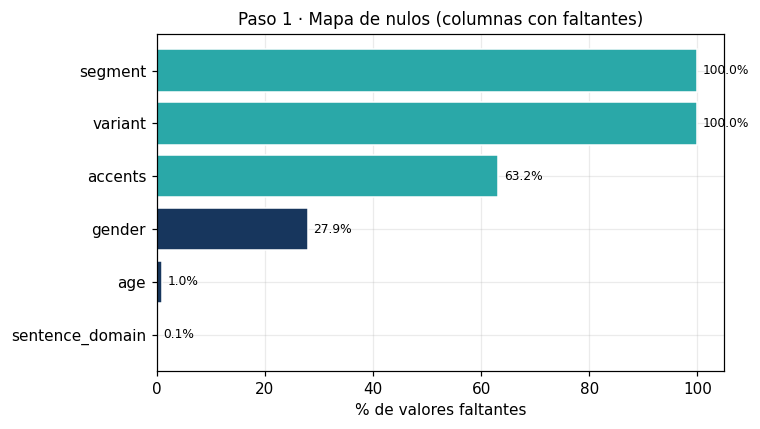
\includegraphics[width=0.72\linewidth]{eda_fig1_nulos.png}
  \caption{Porcentaje de valores faltantes por columna}
  \label{fig:eda-nulos}
  \notaAPA{En turquesa, las columnas inservibles ($\ge$50\,\% de nulos). Elaboraci{\'o}n
  propia.}
\end{figure}

\textbf{Duplicados y fuga potencial.} No hay filas ni audios repetidos, pero solo existen
\textbf{2\,067 frases {\'u}nicas}: cada una se grab{\'o} $\approx$11 veces por distintos
hablantes. No es un defecto ---es lo esperable en un corpus ASR multi-hablante---, pero
obliga a \textbf{particionar por frase o por hablante} para evitar \emph{fuga de datos}
(Secci{\'o}n~\ref{sec:eda-particion}). \textbf{Errores.} La etiqueta \texttt{sentence\_domain}
es multi-valor; 76 filas repiten \emph{tokens} internos y se corrigen deduplicando. Ning{\'u}n
clip validado tiene \texttt{net\_votes}\,$\le$\,0.

\subsubsection{Anatom\'ia num\'erica y desbalances}
\label{sec:eda-anatomia}

El histograma y el diagrama de caja leen los mismos datos de forma distinta: el primero
muestra la \emph{forma} de la distribuci{\'o}n; el segundo, la mediana, la dispersi{\'o}n y
los valores at{\'i}picos (Figuras~\ref{fig:eda-hist} y~\ref{fig:eda-box}). Las
distribuciones son unimodales, con leve asimetr{\'i}a a la derecha, y exhiben colas que
exponen clips extremos en duraci{\'o}n y velocidad.

\begin{figure}[H]
  \centering
  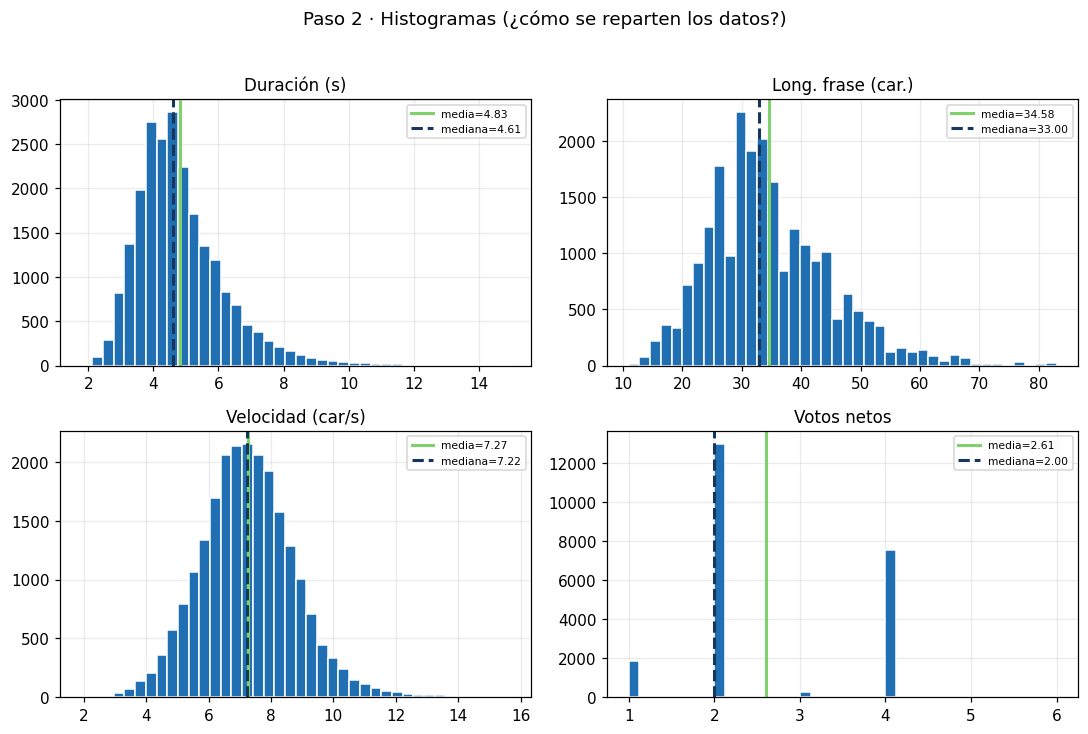
\includegraphics[width=0.82\linewidth]{eda_fig2_histogramas.png}
  \caption{Histogramas de las variables num\'ericas}
  \label{fig:eda-hist}
  \notaAPA{Distribuciones unimodales con leve asimetr{\'i}a a la derecha. Elaboraci{\'o}n
  propia.}
\end{figure}

\begin{figure}[H]
  \centering
  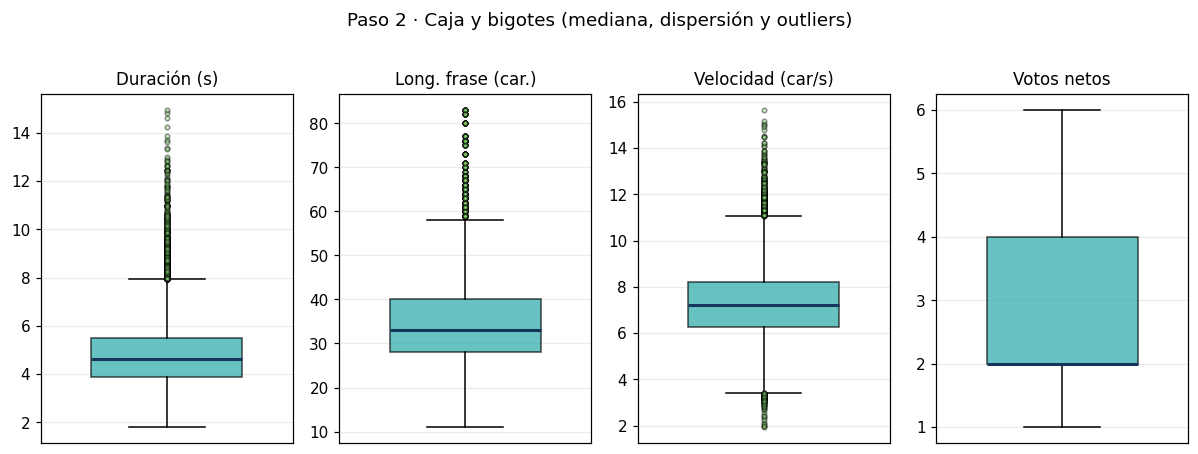
\includegraphics[width=\linewidth]{eda_fig3_boxplots.png}
  \caption{Diagramas de caja y bigotes de las variables num\'ericas}
  \label{fig:eda-box}
  \notaAPA{Las colas de puntos exponen clips extremos de duraci{\'o}n y velocidad
  (desajuste audio--texto). Elaboraci{\'o}n propia.}
\end{figure}

El an{\'a}lisis de las variables categ{\'o}ricas (Figura~\ref{fig:eda-barras}) revela los
hallazgos m{\'a}s importantes del diagn{\'o}stico:

\begin{itemize}\itemsep1pt
  \item \textbf{G{\'e}nero severamente desbalanceado}: 16\,079 \texttt{female} frente a
        solo \textbf{308} \texttt{male} (y 6\,340 \texttt{unknown}). Un modelo entrenado
        as{\'i} aprender{\'a} sobre todo voz femenina: sesgo que debe declararse como
        limitaci{\'o}n para un uso m{\'e}dico con pacientes de ambos sexos.
  \item \textbf{Edad} concentrada en \texttt{twenties} y \texttt{thirties}.
  \item \textbf{Dominio salud}: $\approx$\textbf{78\,\%} de los clips incluyen
        \texttt{healthcare}, cobertura favorable para la tesis m{\'e}dica.
  \item \textbf{Concentraci{\'o}n de hablantes}: un {\'u}nico hablante aporta
        \textbf{8,9\,\%} del corpus (2\,013 clips), lo que refuerza la partici{\'o}n por
        hablante.
\end{itemize}

\begin{figure}[H]
  \centering
  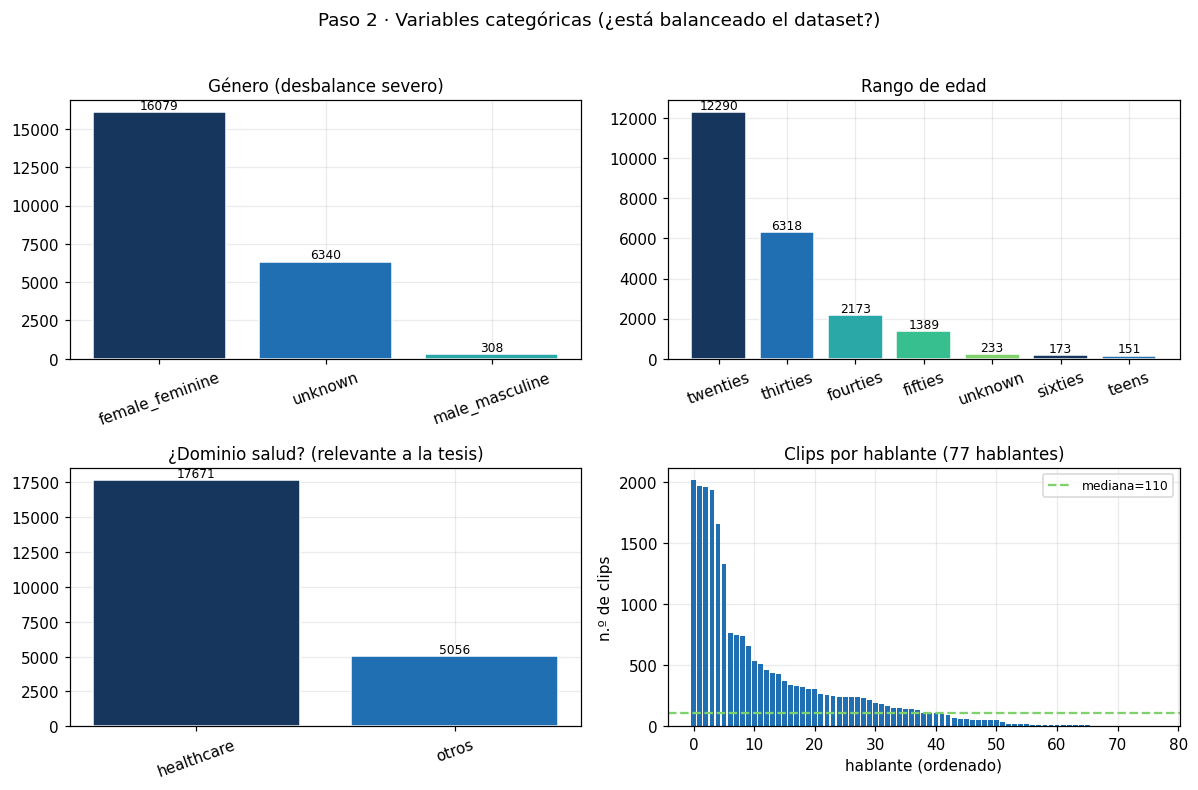
\includegraphics[width=\linewidth]{eda_fig4_barras.png}
  \caption{Distribuci\'on de las variables categ\'oricas del corpus}
  \label{fig:eda-barras}
  \notaAPA{El g{\'e}nero y la concentraci{\'o}n de hablantes son los desbalances
  cr{\'i}ticos. Elaboraci{\'o}n propia.}
\end{figure}

\subsubsection{Correlaciones: Pearson y Spearman}
\label{sec:eda-correlaciones}

La longitud de la frase y la duraci{\'o}n del audio se mueven juntas en diagonal ascendente
(Figura~\ref{fig:eda-disp}): relaci{\'o}n positiva y lineal. La velocidad frente a la
duraci{\'o}n es d{\'e}bilmente negativa, por un efecto de borde en clips muy cortos.

\begin{figure}[H]
  \centering
  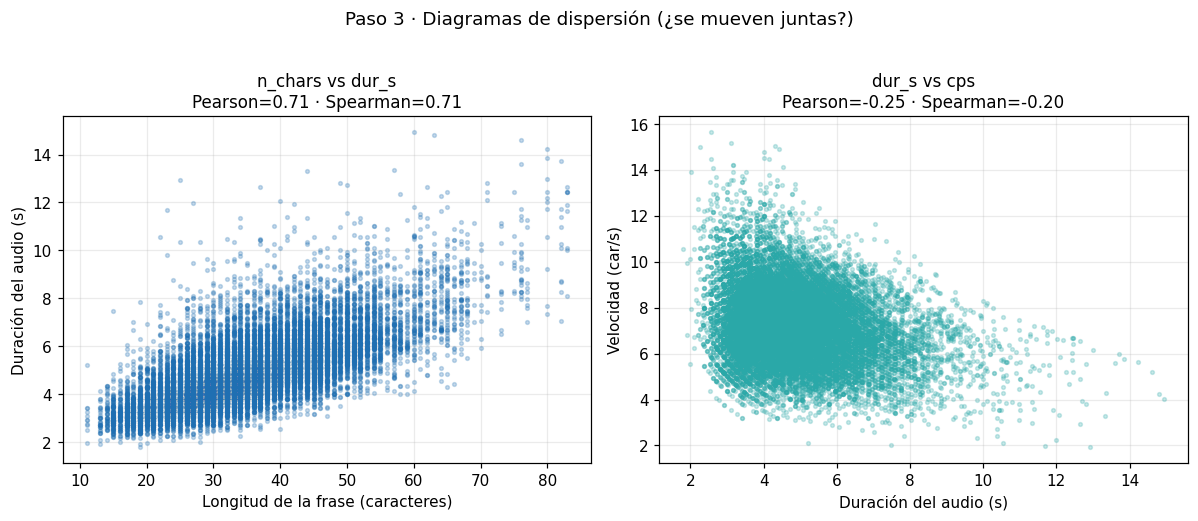
\includegraphics[width=\linewidth]{eda_fig5_dispersion.png}
  \caption{Diagramas de dispersi\'on con sus coeficientes de Pearson y Spearman}
  \label{fig:eda-disp}
  \notaAPA{Elaboraci{\'o}n propia.}
\end{figure}

Se reportan ambos coeficientes (Figura~\ref{fig:eda-heat}): \textbf{Pearson} mide la
asociaci{\'o}n \emph{lineal}; \textbf{Spearman}, basado en rangos, mide la \emph{monoton{\'i}a}
y es robusto a valores at{\'i}picos y a la no-normalidad. Coinciden en relaciones limpias
(\texttt{dur\_s}\,$\sim$\,\texttt{n\_chars}\,$=0{,}71$) pero divergen donde hay asimetr{\'i}a:
\texttt{down\_votes}\,$\sim$\,\texttt{net\_votes} vale $-0{,}37$ (Pearson) frente a $-0{,}50$
(Spearman). Esa diferencia justifica usar ambas m{\'e}tricas y no fiarse de una sola.

\begin{figure}[H]
  \centering
  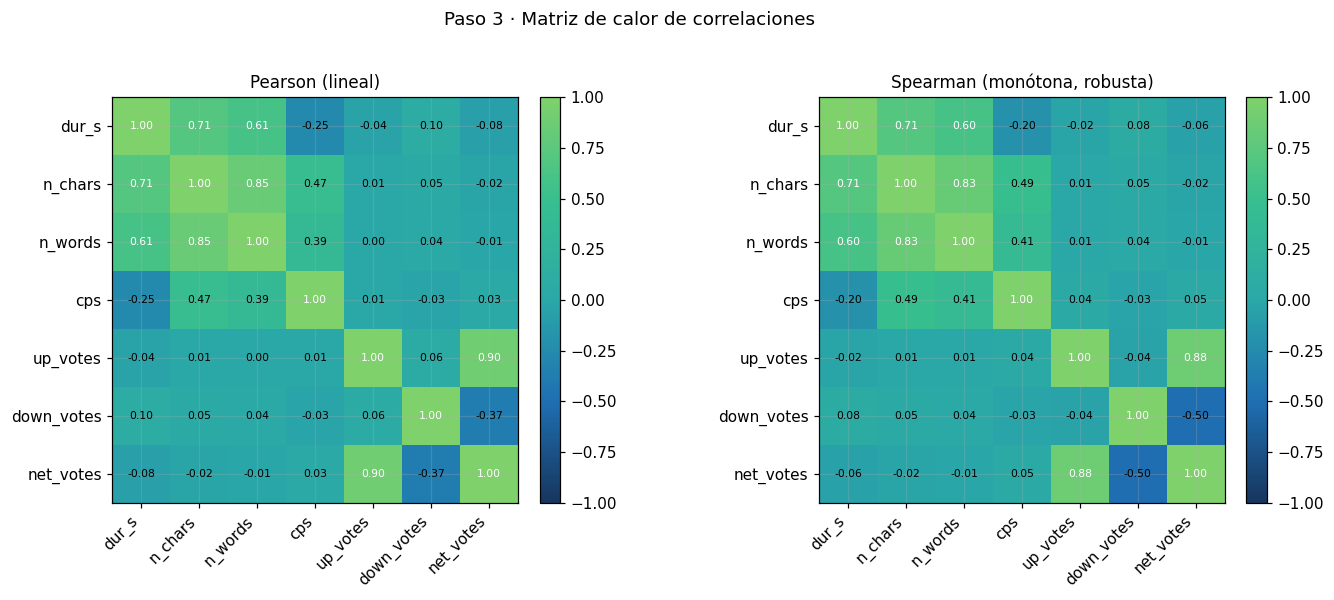
\includegraphics[width=\linewidth]{eda_fig6_heatmaps.png}
  \caption{Matrices de calor de correlaci\'on de Pearson y de Spearman}
  \label{fig:eda-heat}
  \notaAPA{Izquierda: Pearson (lineal). Derecha: Spearman (mon{\'o}tona, robusta).
  Elaboraci{\'o}n propia.}
\end{figure}

\subsubsection{Variable objetivo: dominio de salud}
\label{sec:eda-salud}

Como la investigaci{\'o}n se orienta a la consulta m{\'e}dica, se cruzaron las variables de
forma por el indicador \texttt{is\_healthcare} (Figura~\ref{fig:eda-obj}). El subconjunto de
salud muestra frases algo m{\'a}s cortas (mediana 32 frente a 36 caracteres) y ligeramente
m{\'a}s lentas. Las diferencias son peque{\~n}as pero \textbf{estad{\'i}sticamente
significativas} (prueba de Mann--Whitney, $p \ll 0{,}001$) por el gran tama{\~n}o muestral.
El dominio cl{\'i}nico, que cubre el \textbf{77,8\,\%} del corpus limpio, est{\'a} bien
representado y es homog{\'e}neo con el resto, sin sesgos de forma que dificulten el ajuste.

\begin{figure}[H]
  \centering
  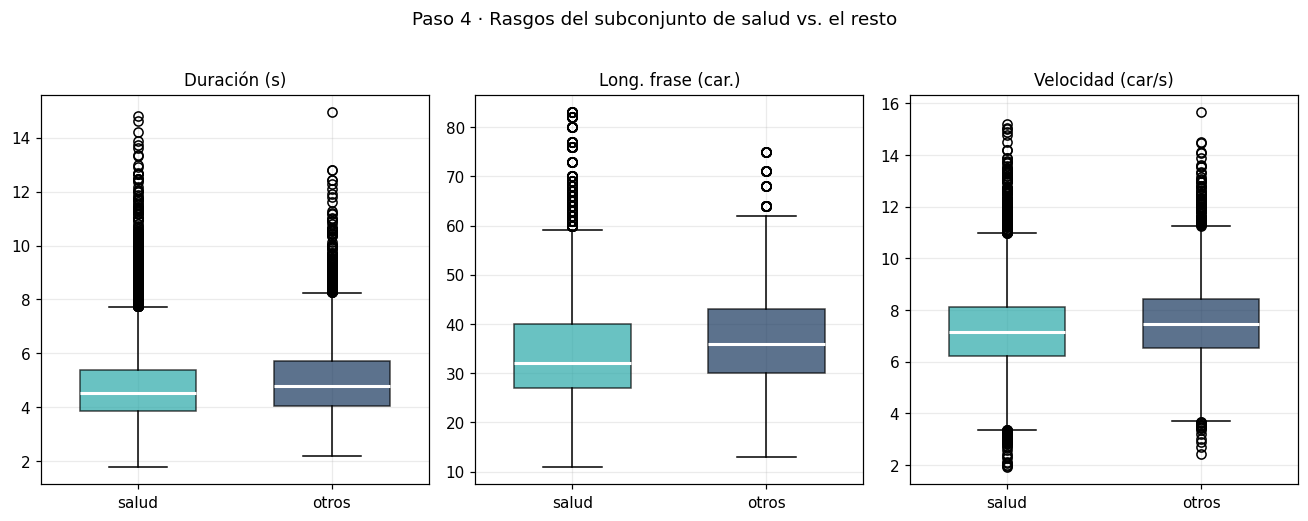
\includegraphics[width=\linewidth]{eda_fig7_objetivo.png}
  \caption{Gr\'aficos cruzados: subconjunto de salud frente al resto del corpus}
  \label{fig:eda-obj}
  \notaAPA{Elaboraci{\'o}n propia.}
\end{figure}

\subsubsection{Dataset limpio resultante}
\label{sec:eda-limpieza}

Respetando el orden del protocolo ---primero limpiar, luego una variable, luego dos y al
final el objetivo--- se obtiene el dataset depurado. El criterio de inclusi{\'o}n para
entrenamiento es: sin valor at{\'i}pico por la regla intercuart{\'i}lica de Tukey en
\texttt{dur\_s} y \texttt{cps}, y \texttt{net\_votes}\,$>$\,0. El corpus pas{\'o} de
\textbf{22\,727} a \textbf{21\,653} clips (Tabla~\ref{tab:eda-limpieza}).

\begin{table}[H]
  \centering
  \caption{Decisiones de limpieza y su efecto sobre el corpus}
  \label{tab:eda-limpieza}
  \small
  \begin{tabularx}{\linewidth}{@{}X r@{}}
    \toprule
    Decisi\'on de limpieza & Efecto \\
    \midrule
    Eliminar columnas vac\'ias, constantes o redundantes & $-4$ columnas \\
    Normalizar \texttt{sentence\_domain} (deduplicar \emph{tokens}) & 76 filas corregidas \\
    Imputar nulos demogr\'aficos como \texttt{unknown} & 0 filas perdidas \\
    Excluir at\'ipicos (IQR) de duraci\'on y velocidad & $-1\,074$ filas (4,7\,\%) \\
    \midrule
    \textbf{Corpus validado crudo} $\rightarrow$ \textbf{dataset limpio} & \textbf{22\,727 $\rightarrow$ 21\,653} \\
    \bottomrule
  \end{tabularx}
  \notaAPA{La regla intercuart{\'i}lica (criterio de Tukey) se aplic{\'o} sobre
  \texttt{dur\_s} y \texttt{cps}. Elaboraci{\'o}n propia.}
\end{table}

\subsubsection{Normalizaci\'on ortogr\'afica del quechua}
\label{sec:eda-normalizacion}

La tasa de error del ASR es sensible a diferencias ortogr{\'a}ficas invisibles en la
referencia. Se fij{\'o} una convenci{\'o}n {\'u}nica y documentada: forma Unicode NFC;
unificaci{\'o}n de las variantes tipogr{\'a}ficas del ap{\'o}strofo al ap{\'o}strofo recto
\texttt{'} ---preservando su valor \emph{fon{\'e}mico} como marca de glotalizaci{\'o}n en
las oclusivas quechuas (\emph{p', t', ch', k', q'})---; conversi{\'o}n a min{\'u}sculas;
retiro de la puntuaci{\'o}n no pronunciada conservando ap{\'o}strofo y gui{\'o}n internos; y
colapso de espacios. La normalizaci{\'o}n afect{\'o} al \textbf{99,9\,\%} de las
transcripciones y redujo las frases {\'u}nicas del dataset limpio de 2\,062 a \textbf{2\,058}
al fundir variantes equivalentes. No se hallaron d{\'i}gitos en el texto, por lo que no fue
necesario desambiguar n{\'u}meros hablados.

\subsubsection{Partici\'on anti-fuga: el \emph{trade-off} hablante\,/\,frase}
\label{sec:eda-particion}

El re{\'u}so masivo de frases obliga a controlar la \emph{fuga de datos}. Se evaluaron los
dos ejes de partici{\'o}n posibles, cada uno disjunto en un eje y midiendo la fuga residual
en el otro (Tabla~\ref{tab:eda-particion}). El hallazgo es que ambos ejes son
\textbf{incompatibles} en este corpus: como casi todos los hablantes graban las mismas
2\,058 frases, una partici{\'o}n disjunta por hablante deja el $\sim$100\,\% de las frases
de prueba tambi{\'e}n en entrenamiento, y una disjunta por frase deja el $\sim$100\,\% de
las voces compartidas.

\begin{table}[H]
  \centering
  \caption{Las dos particiones (80/10/10 por n\'umero de clips) y su fuga residual}
  \label{tab:eda-particion}
  \small
  \begin{tabularx}{\linewidth}{@{}l r r r X@{}}
    \toprule
    Partici\'on & Train & Val & Test & Fuga residual (test) \\
    \midrule
    Disjunta por \textbf{hablante} & 17\,139 & 2\,260 & 2\,254 & 100\,\% de las \emph{frases} ya vistas \\
    Disjunta por \textbf{frase}    & 17\,309 & 2\,168 & 2\,176 & 100\,\% de las \emph{voces} ya vistas \\
    \bottomrule
  \end{tabularx}
  \notaAPA{Semilla \texttt{SEED=42}. Ambas particiones quedan fijadas en columnas
  reproducibles del dataset (\texttt{split\_sentence}, \texttt{split\_speaker}).
  Elaboraci{\'o}n propia.}
\end{table}

Para un ASR m{\'e}dico, cuyo objetivo es transcribir \emph{frases nuevas} dichas en
consulta mediante un modelo de base tipo Whisper \parencite{radford2023whisper}, la
amenaza m{\'a}s grave es que el modelo memorice el repertorio fijo de frases. Por ello se
adopta la \textbf{partici{\'o}n disjunta por frase} como principal, y se conserva la
disjunta por hablante como evaluaci{\'o}n complementaria de robustez ante voces no vistas;
el solapamiento de hablantes se declara como limitaci{\'o}n.

\subsubsection{S\'intesis, rigor e implicaciones}
\label{sec:eda-sintesis}

El EDA entrega un corpus de 21\,653 clips depurados, con texto normalizado y dos
particiones verificadas sin fuga en su eje respectivo. El estudio se apoya en cuatro
dimensiones de rigor: \emph{metodol{\'o}gica} (orden estricto del protocolo; cada decisi{\'o}n
sobre evidencia num{\'e}rica), \emph{te{\'o}rica} (Pearson y Spearman complementarios, regla
IQR de Tukey, contrastes de Mann--Whitney), \emph{interpretativa} (cada figura con su lectura,
distinguiendo hallazgos reales de asociaciones triviales) y \emph{replicabilidad} (semilla
fija, versiones registradas, resultados deterministas).

De este an{\'a}lisis se derivan tres decisiones que gobiernan el resto del cap{\'i}tulo:
(i) evaluar con la partici{\'o}n disjunta por frase y reportar tambi{\'e}n la disjunta por
hablante; (ii) informar la tasa de error \emph{estratificada por g{\'e}nero} para exponer el
sesgo del desbalance 16\,079\,/\,308; y (iii) usar este corpus depurado ---no el crudo---
como base del factor «calidad del corpus» del experimento de ablaci{\'o}n descrito en la
metodolog{\'i}a (Tabla~\ref{tab:ablacion}). Todo el proceso es reproducible mediante los
\emph{scripts} \texttt{eda\_limpieza.py} y \texttt{particionar\_dataset.py} de los Anexos.

% ------------------------------------------------------------
% Las secciones 4.2 (resultados ASR), 4.3 (resultados MT quy->quz),
% 4.4 (resultados TTS) y 4.5 (an{\'a}lisis de error) se completar{\'a}n al ejecutar
% los experimentos. El experimento de ablaci{\'o}n de calidad de corpus ya est{\'a}
% formalizado en el Cap{\'i}tulo III (Tabla~\ref{tab:ablacion}).
% ------------------------------------------------------------
   % Cap. IV - Experimentacion y Resultados (EDA)
% ##################################################################
% CAPÍTULO IV: ESTUDIO DE FACTIBILIDAD
% ##################################################################
\clearpage
\section{Estudio de factibilidad}

\subsection{Enfoque adoptado}
El proyecto es viable porque reutiliza modelos preentrenados de c{\'o}digo abierto (MMS, NLLB,
Whisper) mediante ajuste fino, lo que reduce dr{\'a}sticamente los requisitos de datos y c{\'o}mputo
frente a entrenar desde cero. La factibilidad se analiza en sus dimensiones t{\'e}cnica,
econ{\'o}mica y operativa.

\subsection{Factibilidad t{\'e}cnica}

\subsubsection{Hardware, c{\'o}mputo e inferencia}
El ajuste de modelos preentrenados puede realizarse en una estaci{\'o}n con GPU y complementarse con
cr{\'e}ditos de GPU en la nube para las fases intensivas. La inferencia del \emph{pipeline} integrado
es ejecutable en equipo de gama media, compatible con un piloto en el punto de atenci{\'o}n.
\obscuatro{En concreto, el \emph{fine-tuning} se realiza en \textbf{GPU en la nube} (Colab Pro,
Kaggle o nube institucional) con t{\'e}cnicas de bajo consumo de memoria (\emph{LoRA}/\emph{PEFT}),
dado que el equipo local (WSL2 sin GPU dedicada) se reserva para la inferencia; el presupuesto de
horas-GPU se refleja en la factibilidad econ{\'o}mica.}

\subsubsection{Estrategia de datos}
El cuello de botella es el corpus cl{\'i}nico Quechua--Espa{\~n}ol, que se construir{\'a} de forma
acotada (vocabulario y frases de triaje, s{\'i}ntomas e indicaciones) y se complementar{\'a} con
recursos existentes (\emph{Huqariq}, QuBERT) y datos sint{\'e}ticos cuando sea pertinente.

\subsubsection{Herramientas y software}
Se emplear{\'a}n bibliotecas de c{\'o}digo abierto para habla y traducci{\'o}n (modelos MMS, NLLB y
Whisper de Meta/OpenAI y sus ecosistemas), herramientas de evaluaci{\'o}n (c{\'a}lculo de WER, BLEU y
chrF) y entornos reproducibles de \emph{fine-tuning}.

\subsection{Factibilidad econ{\'o}mica}
El presupuesto estimado (Tabla~\ref{tab:presupuesto}) asciende a \textbf{S/ 7\,350.00}, dominado por
hardware con GPU y cr{\'e}ditos de c{\'o}mputo; es asumible en el marco de un trabajo de tesis y
puede financiarse con recursos propios y/o apoyo institucional.

\subsection{Factibilidad operativa}
La validaci{\'o}n con consultas simuladas y participantes voluntarios evita la dependencia de
aprobaciones cl{\'i}nicas complejas y permite ejecutar los experimentos \obscuatro{dentro del
cronograma anual (12 meses)}, en un centro de salud de referencia en Cusco.

\subsection{\obscuatro{An{\'a}lisis de riesgos y mitigaci{\'o}n}}
\begin{bloqueObsCuatro}
\noindent Los principales riesgos del proyecto y sus medidas de mitigaci{\'o}n se resumen en la
Tabla~\ref{tab:riesgos}; se priorizan por su impacto sobre los objetivos espec{\'i}ficos.
\end{bloqueObsCuatro}

\begin{table}[H]
\centering
\caption{\obscuatro{Matriz de riesgos y mitigaci{\'o}n.}}
\label{tab:riesgos}
\small
\begin{tabularx}{\linewidth}{@{}p{3.5cm} c X@{}}
\toprule\hdr{Riesgo} & \hdr{Prob./Imp.} & \hdr{Mitigaci{\'o}n} \\
\midrule
Corpus cl{\'i}nico insuficiente para el ajuste & Alta / Alto &
Aumento de datos (retrotraducci{\'o}n, sint{\'e}ticos) y reuso de \emph{Huqariq}/QuBERT; el corpus se usa sobre todo como \emph{benchmark}. \\
Escasa disponibilidad de hablantes nativos \sig{quz} & Media / Alto &
Convocatoria temprana de voluntarios biling{\"u}es; validaci{\'o}n por paneles reducidos ($\ge$ 3 revisores). \\
Latencia del \emph{pipeline} superior a la meta & Media / Medio &
Modelos ligeros, cuantizaci{\'o}n y evaluaci{\'o}n por etapas (presupuesto de la Tabla~\ref{tab:latencias}). \\
Costo/acceso a GPU en la nube & Media / Medio &
\emph{LoRA}/\emph{PEFT} y precisi{\'o}n reducida; cr{\'e}ditos gratuitos (Colab/Kaggle) y nube institucional. \\
Baja ganancia dialectal \sig{quy}$\to$\sig{quz} & Media / Alto &
Segmentaci{\'o}n morfol{\'o}gica, validaci{\'o}n con nativos y l{\'i}neas base de comparaci{\'o}n. \\
\bottomrule
\end{tabularx}
\notaAPA{\obscuatro{Elaboraci{\'o}n propia. Prob./Imp.: probabilidad e impacto estimados.}}
\end{table}

\subsection{Viabilidad y sostenibilidad}
El proceso (corpus + ajuste + evaluaci{\'o}n) es replicable en otras variantes del quechua o en otros
dominios, y el uso de modelos de c{\'o}digo abierto favorece la continuidad y la apropiaci{\'o}n local
de la tecnolog{\'i}a.
       % Cap. V  - Factibilidad
% ##################################################################
% CAPÍTULO V: ASPECTOS ADMINISTRATIVOS
% ##################################################################
\clearpage
\section{Aspectos administrativos}

\subsection{Cronograma de actividades}
El proyecto se ejecuta en \textbf{12 meses (octubre 2026 -- septiembre 2027)}, organizado por meses.
La Tabla~\ref{tab:cronograma} presenta el diagrama de Gantt, con las actividades agrupadas en tres
fases ---\emph{administrativa}, de \emph{desarrollo} (ASR, MT y TTS) e \emph{investigaci{\'o}n y
cierre}---; los m{\'o}dulos ASR, MT y TTS se ejecutan de forma parcialmente paralela mediante el
ajuste de modelos preentrenados.

% ----- gris de la fase administrativa -----
\definecolor{adminG}{HTML}{8A98A6}
% \gbar{fila}{semana inicial}{semana final}{color}{etiqueta}
\newcommand{\gbar}[5]{%
  \fill[#4,rounded corners=2.2pt] ({#2-1},{-#1+1-0.20}) rectangle ({#3},{-#1+1+0.20});%
  \node[anchor=west,align=left,text width=4.9cm,font=\scriptsize,text=black!80]
       at (-8.2,{-#1+1}) {#5};}

\begin{table}[H]
\caption{Cronograma de actividades (octubre 2026 -- septiembre 2027), por meses.}
\label{tab:cronograma}

% ----- leyenda de fases (alineada a la izquierda) -----
\noindent{\scriptsize
\begin{tikzpicture}[baseline]
  \fill[adminG,rounded corners=1.5pt](0,0) rectangle (0.32,0.26);
  \node[anchor=west] at (0.4,0.13) {Administrativo};
  \fill[g3,rounded corners=1.5pt](3.0,0) rectangle (3.32,0.26);
  \node[anchor=west] at (3.4,0.13) {Desarrollo (ASR, MT, TTS)};
  \fill[g10,rounded corners=1.5pt](7.6,0) rectangle (7.92,0.26);
  \node[anchor=west] at (8.0,0.13) {Investigaci{\'o}n y cierre};
\end{tikzpicture}}

\smallskip
\noindent\resizebox{\linewidth}{!}{%
\begin{tikzpicture}[x=0.92cm,y=0.82cm,font=\scriptsize]
  % --- banda de meses (navy): 12 meses, oct 2026 -> sep 2027 ---
  \fill[g5,rounded corners=1.5pt] (0,0.74) rectangle (12,1.6);
  \foreach \m/\pos in {Oct/0.5,Nov/1.5,Dic/2.5,Ene/3.5,Feb/4.5,Mar/5.5,Abr/6.5,May/7.5,Jun/8.5,Jul/9.5,Ago/10.5,Sep/11.5}
     \node[white,font=\bfseries\scriptsize] at (\pos,1.17) {\m};
  % --- numeros de mes (1..12) ---
  \foreach \w in {1,...,12}
     \node[font=\tiny,text=black!55] at ({\w-0.5},0.45) {\w};
  % --- separadores de mes ---
  \foreach \xg in {0,...,12}
     \draw[black!18,very thin] (\xg,0.74) -- (\xg,-12.6);
  % --- lineas horizontales entre filas ---
  \foreach \r in {0,...,13}
     \draw[black!10,very thin] (0,{-\r+0.5}) -- (12,{-\r+0.5});
  % --- barras (fila, mes inicial, mes final, color, etiqueta) ---
  \gbar{1}{1}{1}{adminG}{Aprobaci{\'o}n del plan de tesis}
  \gbar{2}{1}{3}{g1}{Revisi{\'o}n del estado del arte}
  \gbar{3}{2}{4}{g2}{Recolecci{\'o}n y preparaci{\'o}n del corpus (salud)}
  \gbar{4}{4}{5}{g7}{\textbf{Validaci{\'o}n del corpus con hablantes nativos (hito cr{\'i}tico)}}
  \gbar{5}{5}{6}{g3}{M{\'o}dulo ASR (voz $\to$ texto)}
  \gbar{6}{5}{7}{g4}{M{\'o}dulo MT (traducci{\'o}n, aporte central)}
  \gbar{7}{6}{8}{g5}{M{\'o}dulo TTS (texto $\to$ voz)}
  \gbar{8}{8}{9}{g6}{Integraci{\'o}n del \emph{pipeline}}
  \gbar{9}{9}{10}{g8}{Evaluaci{\'o}n experimental (WER, BLEU, MOS) y ablaci{\'o}n}
  \gbar{10}{10}{11}{g9}{Validaci{\'o}n m{\'e}dico-paciente (simulada)}
  \gbar{11}{11}{11}{g10}{An{\'a}lisis de resultados}
  \gbar{12}{10}{12}{g11}{Redacci{\'o}n del informe final}
  \gbar{13}{12}{12}{g12}{Sustentaci{\'o}n}
\end{tikzpicture}}
\notaAPA{Elaboraci{\'o}n propia. Cada columna representa un mes (octubre 2026 -- septiembre 2027); el color identifica la fase y el solapamiento de las barras refleja el desarrollo parcialmente paralelo de los m{\'o}dulos ASR, MT y TTS. La \textbf{validaci{\'o}n del corpus con hablantes nativos} se destaca como \emph{hito cr{\'i}tico}: condiciona el ajuste del m{\'o}dulo de traducci{\'o}n ---aporte central--- y es la entrada que distingue este proyecto del antecedente m{\'a}s cercano.}
\end{table}

\subsection{Presupuesto y financiamiento}
La Tabla~\ref{tab:presupuesto} resume los recursos estimados para el desarrollo del proyecto.

\begin{table}[H]
\centering
\caption{Recursos para el desarrollo del proyecto de tesis (soles).}
\label{tab:presupuesto}
\small
\begin{tabularx}{\linewidth}{@{}l X r@{}}
\toprule\hdr{Tipo} & \hdr{Descripci{\'o}n} & \hdr{Costo (S/)} \\
\midrule
Hardware & Laptop/PC con GPU (entrenamiento y \emph{fine-tuning}) & 4\,500.00 \\
C{\'o}mputo & Cr{\'e}ditos de GPU en la nube (horas de ajuste) & 900.00 \\
Datos & Grabaci{\'o}n y \textbf{validaci{\'o}n experta del corpus cl{\'i}nico} por hablantes nativos (insumo cr{\'i}tico del aporte: incentivos y sesiones de validaci{\'o}n) & 1\,200.00 \\
Administrativos & Impresiones, inscripci{\'o}n y tr{\'a}mites de tesis & 600.00 \\
Movilidad & Traslados al centro de salud y a comunidades & 300.00 \\
Otros & Gastos no previstos & 250.00 \\
\multicolumn{2}{@{}l}{\textbf{Total}} & \textbf{7\,750.00} \\
\bottomrule
\end{tabularx}
\notaAPA{Montos estimados en soles (S/). Elaboraci{\'o}n propia. La partida de \emph{datos} prioriza la validaci{\'o}n del corpus por hablantes nativos ---insumo cr{\'i}tico del aporte central--- conforme al hito destacado en el cronograma (Tabla~\ref{tab:cronograma}).}
\end{table}

\subsection{Equipo de investigaci{\'o}n}
La Tabla~\ref{tab:equipo} detalla el equipo responsable del proyecto.

\begin{table}[H]
\centering
\caption{Equipo de investigaci{\'o}n.}
\label{tab:equipo}
\small
\begin{tabularx}{\linewidth}{@{}l X@{}}
\toprule\hdr{Rol} & \hdr{Responsable / funci{\'o}n} \\
\midrule
Tesista   & Alain Armando Condori Contreras ---dise{\~n}o, desarrollo y evaluaci{\'o}n del sistema---. \\
Asesor    & Mtro. Ing. Ra{\'u}l Huillca Huallparimachi ---orientaci{\'o}n metodol{\'o}gica y t{\'e}cnica---. \\
Colaboradores & Personal de salud biling{\"u}e (validaci{\'o}n del corpus) y participantes voluntarios (consultas simuladas). \\
\bottomrule
\end{tabularx}
\notaAPA{Elaboraci{\'o}n propia. Los colaboradores intervienen en la validaci{\'o}n del corpus y en la actuaci{\'o}n de las consultas simuladas.}
\end{table}
    % Cap. VI - Aspectos administrativos

% ---- Cierre ----
% ================= BIBLIOGRAFÍA =================
\newpage
\defbibnote{vigencia}{\footnotesize\textit{Nota sobre la vigencia de las fuentes.}
Se priorizaron publicaciones de los {\'u}ltimos cinco a{\~n}os (2021--2026). Las referencias
anteriores se conservan por ser (a)~obras \emph{seminales} que definen los m{\'e}todos empleados
---el \emph{Transformer} \parencite{vaswani2017attention}, BLEU \parencite{papineni2002bleu} y chrF
\parencite{popovic2015chrf}---; (b)~\emph{libros} de metodolog{\'i}a en su edici{\'o}n vigente
\parencite{hernandez2018metodologia}; y (c)~\emph{fuentes primarias oficiales} o trabajos
fundacionales del PLN para el quechua ---los Censos Nacionales \parencite{inei2017} y los primeros
sistemas de traducci{\'o}n \parencite{ortega2020quechua} y reconocimiento de voz
\parencite{Zevallos202061} para esta lengua---.\par\vspace{4pt}}
\printbibliography[heading=bibintoc,title={Referencias},prenote=vigencia]
    % Referencias (APA7)
% ================= ANEXOS =================
\newpage
\section*{Anexos}
\addcontentsline{toc}{section}{Anexos}

% ----- Anexo 1 -----
\subsection*{Anexo 1: Ficha t{\'e}cnica de registro experimental}
\addcontentsline{toc}{subsection}{Anexo 1: Ficha t{\'e}cnica de registro experimental}
Plantilla para registrar cada \emph{turno de traducci{\'o}n} durante las consultas simuladas.

\begin{table}[H]
\centering
\caption{Ficha t{\'e}cnica de registro por turno (plantilla).}
\label{tab:ficha}
\small
\begin{tabularx}{\linewidth}{@{}l X@{}}
\toprule\hdr{Campo} & \hdr{Valor registrado} \\
\midrule
ID de turno / sesi{\'o}n            & \rule{5cm}{0.3pt} \\
Escenario (triaje/s{\'i}ntomas/indicaciones) & \rule{5cm}{0.3pt} \\
Direcci{\'o}n (\sig{quz}$\to$es / es$\to$\sig{quz}) & \rule{5cm}{0.3pt} \\
Transcripci{\'o}n ASR / WER         & \rule{5cm}{0.3pt} \\
Traducci{\'o}n MT / BLEU / chrF     & \rule{5cm}{0.3pt} \\
Calidad de voz (MOS)               & \rule{5cm}{0.3pt} \\
Latencia por turno (s)             & \rule{5cm}{0.3pt} \\
Observaciones                      & \rule{5cm}{0.3pt} \\
\bottomrule
\end{tabularx}
\notaAPA{Elaboraci{\'o}n propia. Se completa una ficha por cada turno de traducci{\'o}n registrado.}
\end{table}

% ----- Anexo 2 -----
\subsection*{Anexo 2: Plantilla del banco de frases de consulta (evaluaci{\'o}n)}
\addcontentsline{toc}{subsection}{Anexo 2: Plantilla del banco de frases de consulta (evaluaci{\'o}n)}
Gui{\'o}n base de frases por escenario; el equivalente en quechua de Cusco se valida con hablantes
nativos antes de su uso.

\begin{table}[H]
\centering
\caption{Banco de frases de consulta simulada (ejemplos; \sig{quz} por validar).}
\label{tab:banco}
\small
\begin{tabularx}{\linewidth}{@{}l X l@{}}
\toprule\hdr{Categor{\'i}a} & \hdr{Enunciado (espa{\~n}ol)} & \hdr{Equivalente (\sig{quz})} \\
\midrule
Triaje       & {\textquestiondown}Qu{\'e} lo trae a la consulta?          & [por validar] \\
Triaje       & {\textquestiondown}Hace cu{\'a}nto tiempo se siente mal?    & [por validar] \\
S{\'i}ntomas & {\textquestiondown}D{\'o}nde le duele?                      & [por validar] \\
S{\'i}ntomas & {\textquestiondown}Tiene fiebre o escalofr{\'i}os?          & [por validar] \\
Indicaciones & Tome esta pastilla cada 8 horas.                          & [por validar] \\
Indicaciones & Regrese en 3 d{\'i}as si no mejora.                        & [por validar] \\
\bottomrule
\end{tabularx}
\notaAPA{Elaboraci{\'o}n propia. El equivalente en quechua de Cusco (\sig{quz}) se valida con hablantes nativos antes de su uso.}
\end{table}

% ----- Anexo 3 -----
\subsection*{Anexo 3: Cuestionario de percepci{\'o}n (escala Likert)}
\addcontentsline{toc}{subsection}{Anexo 3: Cuestionario de percepci{\'o}n (escala Likert)}
Escala de 1 (\emph{totalmente en desacuerdo}) a 5 (\emph{totalmente de acuerdo}); se aplica al
personal y a los pacientes-actores.

\begin{table}[H]
\centering
\caption{{\'I}tems del cuestionario de percepci{\'o}n.}
\label{tab:likert}
\small
\begin{tabularx}{\linewidth}{@{}c X c@{}}
\toprule\hdr{N.\textordmasculine} & \hdr{{\'I}tem} & \hdr{1--5} \\
\midrule
1 & El sistema facilit{\'o} la comunicaci{\'o}n durante la consulta.     & \rule{1.6cm}{0.3pt} \\
2 & Conf{\'i}o en la traducci{\'o}n que entreg{\'o} el sistema.          & \rule{1.6cm}{0.3pt} \\
3 & Comprend{\'i} con claridad las indicaciones m{\'e}dicas.            & \rule{1.6cm}{0.3pt} \\
4 & La voz sintetizada fue clara y natural.                             & \rule{1.6cm}{0.3pt} \\
5 & El tiempo de respuesta del sistema fue adecuado.                    & \rule{1.6cm}{0.3pt} \\
6 & Usar{\'i}a el sistema en una consulta real.                         & \rule{1.6cm}{0.3pt} \\
\bottomrule
\end{tabularx}
\notaAPA{Elaboraci{\'o}n propia. Escala Likert de 1 (totalmente en desacuerdo) a 5 (totalmente de acuerdo).}
\end{table}

% ----- Anexo 4 -----
\subsection*{Anexo 4: Modelo de consentimiento informado}
\addcontentsline{toc}{subsection}{Anexo 4: Modelo de consentimiento informado}
\noindent\textit{Yo, \rule{5cm}{0.3pt}, declaro haber sido informado(a) sobre los objetivos del
estudio ``\nuevo{Desarrollo de un sistema bidireccional de traducci{\'o}n de voz Quechua--Espa{\~n}ol
mediante \obstitulo{arquitecturas de transformadores multimodales} para consultas m{\'e}dicas en Cusco}''. Entiendo que participar{\'e} de forma voluntaria en consultas
\textbf{simuladas} ---sin datos cl{\'i}nicos reales---, que las grabaciones ser{\'a}n anonimizadas y
usadas solo con fines de investigaci{\'o}n, y que puedo retirarme en cualquier momento sin
perjuicio.}

\vspace{1.2cm}
\noindent\rule{6cm}{0.3pt}\hfill\rule{4cm}{0.3pt}\\
\noindent Firma del participante \hfill Fecha

          % Anexos

\end{document}
